\documentclass[twoside]{book}

% Packages required by doxygen
\usepackage{fixltx2e}
\usepackage{calc}
\usepackage{doxygen}
\usepackage[export]{adjustbox} % also loads graphicx
\usepackage{graphicx}
\usepackage[utf8]{inputenc}
\usepackage{makeidx}
\usepackage{multicol}
\usepackage{multirow}
\PassOptionsToPackage{warn}{textcomp}
\usepackage{textcomp}
\usepackage[nointegrals]{wasysym}
\usepackage[table]{xcolor}

% Font selection
\usepackage[T1]{fontenc}
\usepackage[scaled=.90]{helvet}
\usepackage{courier}
\usepackage{amssymb}
\usepackage{sectsty}
\renewcommand{\familydefault}{\sfdefault}
\allsectionsfont{%
  \fontseries{bc}\selectfont%
  \color{darkgray}%
}
\renewcommand{\DoxyLabelFont}{%
  \fontseries{bc}\selectfont%
  \color{darkgray}%
}
\newcommand{\+}{\discretionary{\mbox{\scriptsize$\hookleftarrow$}}{}{}}

% Page & text layout
\usepackage{geometry}
\geometry{%
  a4paper,%
  top=2.5cm,%
  bottom=2.5cm,%
  left=2.5cm,%
  right=2.5cm%
}
\tolerance=750
\hfuzz=15pt
\hbadness=750
\setlength{\emergencystretch}{15pt}
\setlength{\parindent}{0cm}
\setlength{\parskip}{3ex plus 2ex minus 2ex}
\makeatletter
\renewcommand{\paragraph}{%
  \@startsection{paragraph}{4}{0ex}{-1.0ex}{1.0ex}{%
    \normalfont\normalsize\bfseries\SS@parafont%
  }%
}
\renewcommand{\subparagraph}{%
  \@startsection{subparagraph}{5}{0ex}{-1.0ex}{1.0ex}{%
    \normalfont\normalsize\bfseries\SS@subparafont%
  }%
}
\makeatother

% Headers & footers
\usepackage{fancyhdr}
\pagestyle{fancyplain}
\fancyhead[LE]{\fancyplain{}{\bfseries\thepage}}
\fancyhead[CE]{\fancyplain{}{}}
\fancyhead[RE]{\fancyplain{}{\bfseries\leftmark}}
\fancyhead[LO]{\fancyplain{}{\bfseries\rightmark}}
\fancyhead[CO]{\fancyplain{}{}}
\fancyhead[RO]{\fancyplain{}{\bfseries\thepage}}
\fancyfoot[LE]{\fancyplain{}{}}
\fancyfoot[CE]{\fancyplain{}{}}
\fancyfoot[RE]{\fancyplain{}{\bfseries\scriptsize Generated by Doxygen }}
\fancyfoot[LO]{\fancyplain{}{\bfseries\scriptsize Generated by Doxygen }}
\fancyfoot[CO]{\fancyplain{}{}}
\fancyfoot[RO]{\fancyplain{}{}}
\renewcommand{\footrulewidth}{0.4pt}
\renewcommand{\chaptermark}[1]{%
  \markboth{#1}{}%
}
\renewcommand{\sectionmark}[1]{%
  \markright{\thesection\ #1}%
}

% Indices & bibliography
\usepackage{natbib}
\usepackage[titles]{tocloft}
\setcounter{tocdepth}{3}
\setcounter{secnumdepth}{5}
\makeindex

% Hyperlinks (required, but should be loaded last)
\usepackage{ifpdf}
\ifpdf
  \usepackage[pdftex,pagebackref=true]{hyperref}
\else
  \usepackage[ps2pdf,pagebackref=true]{hyperref}
\fi
\hypersetup{%
  colorlinks=true,%
  linkcolor=blue,%
  citecolor=blue,%
  unicode%
}

% Custom commands
\newcommand{\clearemptydoublepage}{%
  \newpage{\pagestyle{empty}\cleardoublepage}%
}

\usepackage{caption}
\captionsetup{labelsep=space,justification=centering,font={bf},singlelinecheck=off,skip=4pt,position=top}

%===== C O N T E N T S =====

\begin{document}

% Titlepage & ToC
\hypersetup{pageanchor=false,
             bookmarksnumbered=true,
             pdfencoding=unicode
            }
\pagenumbering{alph}
\begin{titlepage}
\vspace*{7cm}
\begin{center}%
{\Large Vapid\+Tetris }\\
\vspace*{1cm}
{\large Generated by Doxygen 1.8.13}\\
\end{center}
\end{titlepage}
\clearemptydoublepage
\pagenumbering{roman}
\tableofcontents
\clearemptydoublepage
\pagenumbering{arabic}
\hypersetup{pageanchor=true}

%--- Begin generated contents ---
\chapter{Vapid\+Tetris}
\label{md_README}
\Hypertarget{md_README}
Poor Tetris game. 
\chapter{Data Structure Index}
\section{Data Structures}
Here are the data structures with brief descriptions\+:\begin{DoxyCompactList}
\item\contentsline{section}{\hyperlink{structcontainer}{container} }{\pageref{structcontainer}}{}
\end{DoxyCompactList}

\chapter{File Index}
\section{File List}
Here is a list of all files with brief descriptions\+:\begin{DoxyCompactList}
\item\contentsline{section}{\hyperlink{container_8c}{container.\+c} }{\pageref{container_8c}}{}
\item\contentsline{section}{\hyperlink{head_8h}{head.\+h} }{\pageref{head_8h}}{}
\item\contentsline{section}{\hyperlink{main_8c}{main.\+c} }{\pageref{main_8c}}{}
\item\contentsline{section}{\hyperlink{mainSDL_8c}{main\+S\+D\+L.\+c} }{\pageref{mainSDL_8c}}{}
\item\contentsline{section}{\hyperlink{update_8c}{update.\+c} }{\pageref{update_8c}}{}
\item\contentsline{section}{\hyperlink{user_8c}{user.\+c} }{\pageref{user_8c}}{}
\end{DoxyCompactList}

\chapter{Data Structure Documentation}
\hypertarget{structcell}{}\section{cell Struct Reference}
\label{structcell}\index{cell@{cell}}
\subsection*{Data Fields}
\begin{DoxyCompactItemize}
\item 
S\+D\+L\+\_\+\+Rect \hyperlink{structcell_ae289d5dfc43a03b47de6dffa417776df}{border}
\item 
S\+D\+L\+\_\+\+Rect \hyperlink{structcell_af2fb9745b37f309905e02fed903748a5}{cases}
\item 
S\+D\+L\+\_\+\+Color \hyperlink{structcell_a17634ccb0012ada2dc1f042314d35c21}{color}
\item 
Uint8 \hyperlink{structcell_a8cefee0153ea06b2465c1142c467b3e0}{r}
\item 
Uint8 \hyperlink{structcell_ac8a350a38ff279748cfe301a30c8878f}{g}
\item 
Uint8 \hyperlink{structcell_a370fd46cdbe470096b56b9c53941eb0e}{b}
\end{DoxyCompactItemize}


\subsection{Detailed Description}


Definition at line 4 of file main\+S\+D\+L.\+c.



\subsection{Field Documentation}
\mbox{\Hypertarget{structcell_a370fd46cdbe470096b56b9c53941eb0e}\label{structcell_a370fd46cdbe470096b56b9c53941eb0e}} 
\index{cell@{cell}!b@{b}}
\index{b@{b}!cell@{cell}}
\subsubsection{\texorpdfstring{b}{b}}
{\footnotesize\ttfamily Uint8 cell\+::b}



Definition at line 8 of file main\+S\+D\+L.\+c.



Referenced by sdl\+Update\+Display().

\mbox{\Hypertarget{structcell_ae289d5dfc43a03b47de6dffa417776df}\label{structcell_ae289d5dfc43a03b47de6dffa417776df}} 
\index{cell@{cell}!border@{border}}
\index{border@{border}!cell@{cell}}
\subsubsection{\texorpdfstring{border}{border}}
{\footnotesize\ttfamily S\+D\+L\+\_\+\+Rect cell\+::border}



Definition at line 5 of file main\+S\+D\+L.\+c.



Referenced by init\+Display(), and sdl\+Display().

\mbox{\Hypertarget{structcell_af2fb9745b37f309905e02fed903748a5}\label{structcell_af2fb9745b37f309905e02fed903748a5}} 
\index{cell@{cell}!cases@{cases}}
\index{cases@{cases}!cell@{cell}}
\subsubsection{\texorpdfstring{cases}{cases}}
{\footnotesize\ttfamily S\+D\+L\+\_\+\+Rect cell\+::cases}



Definition at line 6 of file main\+S\+D\+L.\+c.



Referenced by init\+Display(), and sdl\+Display().

\mbox{\Hypertarget{structcell_a17634ccb0012ada2dc1f042314d35c21}\label{structcell_a17634ccb0012ada2dc1f042314d35c21}} 
\index{cell@{cell}!color@{color}}
\index{color@{color}!cell@{cell}}
\subsubsection{\texorpdfstring{color}{color}}
{\footnotesize\ttfamily S\+D\+L\+\_\+\+Color cell\+::color}



Definition at line 7 of file main\+S\+D\+L.\+c.

\mbox{\Hypertarget{structcell_ac8a350a38ff279748cfe301a30c8878f}\label{structcell_ac8a350a38ff279748cfe301a30c8878f}} 
\index{cell@{cell}!g@{g}}
\index{g@{g}!cell@{cell}}
\subsubsection{\texorpdfstring{g}{g}}
{\footnotesize\ttfamily Uint8 cell\+::g}



Definition at line 8 of file main\+S\+D\+L.\+c.



Referenced by sdl\+Update\+Display().

\mbox{\Hypertarget{structcell_a8cefee0153ea06b2465c1142c467b3e0}\label{structcell_a8cefee0153ea06b2465c1142c467b3e0}} 
\index{cell@{cell}!r@{r}}
\index{r@{r}!cell@{cell}}
\subsubsection{\texorpdfstring{r}{r}}
{\footnotesize\ttfamily Uint8 cell\+::r}



Definition at line 8 of file main\+S\+D\+L.\+c.



Referenced by sdl\+Update\+Display().



The documentation for this struct was generated from the following file\+:\begin{DoxyCompactItemize}
\item 
\hyperlink{mainSDL_8c}{main\+S\+D\+L.\+c}\end{DoxyCompactItemize}

\hypertarget{structcontainer}{}\section{container Struct Reference}
\label{structcontainer}\index{container@{container}}


{\ttfamily \#include $<$head.\+h$>$}

\subsection*{Data Fields}
\begin{DoxyCompactItemize}
\item 
char $\ast$ \hyperlink{structcontainer_aefae69762fe9c24169e2ca5418a711a1}{data}
\item 
int \hyperlink{structcontainer_a1e938d250074e70b9778df1b59121744}{size}
\item 
int \hyperlink{structcontainer_a0069496fb95c879cd33fb79ab726e81a}{len}
\end{DoxyCompactItemize}


\subsection{Detailed Description}


Definition at line 14 of file head.\+h.



\subsection{Field Documentation}
\mbox{\Hypertarget{structcontainer_aefae69762fe9c24169e2ca5418a711a1}\label{structcontainer_aefae69762fe9c24169e2ca5418a711a1}} 
\index{container@{container}!data@{data}}
\index{data@{data}!container@{container}}
\subsubsection{\texorpdfstring{data}{data}}
{\footnotesize\ttfamily char$\ast$ container\+::data}



Definition at line 15 of file head.\+h.



Referenced by check\+Collision(), create\+Cross(), create\+Dot(), create\+L1(), create\+L2(), create\+Line(), create\+U(), delete\+Col(), delete\+Container(), delete\+Row(), display(), full\+Col(), full\+Row(), gravity(), init\+Container(), place(), rotate\+\_\+180(), and rotate\+\_\+90().

\mbox{\Hypertarget{structcontainer_a0069496fb95c879cd33fb79ab726e81a}\label{structcontainer_a0069496fb95c879cd33fb79ab726e81a}} 
\index{container@{container}!len@{len}}
\index{len@{len}!container@{container}}
\subsubsection{\texorpdfstring{len}{len}}
{\footnotesize\ttfamily int container\+::len}



Definition at line 17 of file head.\+h.



Referenced by check\+Collision(), delete\+Col(), delete\+Row(), detect\+Col(), detect\+Row(), display(), full\+Col(), full\+Row(), gravity(), init\+Container(), place(), rotate\+\_\+180(), and rotate\+\_\+90().

\mbox{\Hypertarget{structcontainer_a1e938d250074e70b9778df1b59121744}\label{structcontainer_a1e938d250074e70b9778df1b59121744}} 
\index{container@{container}!size@{size}}
\index{size@{size}!container@{container}}
\subsubsection{\texorpdfstring{size}{size}}
{\footnotesize\ttfamily int container\+::size}



Definition at line 16 of file head.\+h.



Referenced by check\+Collision(), delete\+Col(), detect\+Row(), display(), full\+Col(), gravity(), init\+Container(), place(), rotate\+\_\+180(), and rotate\+\_\+90().



The documentation for this struct was generated from the following file\+:\begin{DoxyCompactItemize}
\item 
\hyperlink{head_8h}{head.\+h}\end{DoxyCompactItemize}

\chapter{File Documentation}
\hypertarget{container_8c}{}\section{container.\+c File Reference}
\label{container_8c}\index{container.\+c@{container.\+c}}
{\ttfamily \#include \char`\"{}head.\+h\char`\"{}}\newline
Include dependency graph for container.\+c\+:
\nopagebreak
\begin{figure}[H]
\begin{center}
\leavevmode
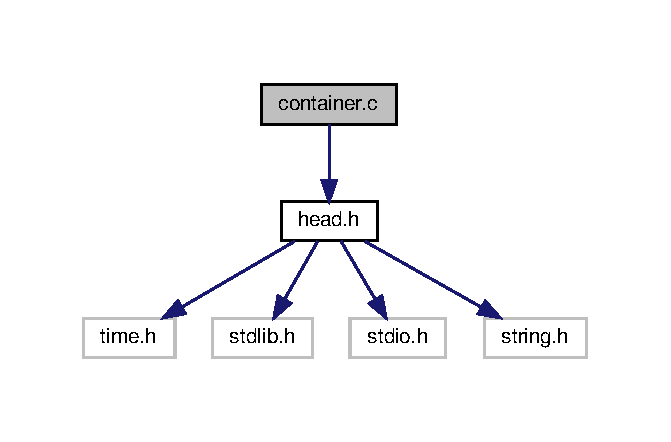
\includegraphics[width=322pt]{container_8c__incl}
\end{center}
\end{figure}
\subsection*{Functions}
\begin{DoxyCompactItemize}
\item 
void \hyperlink{container_8c_af20cf8b598b78389dff22b3d176a3727}{init\+Container} (int width, int height, \hyperlink{structcontainer}{container} $\ast$item)
\item 
\hyperlink{structcontainer}{container} \hyperlink{container_8c_aae1449e449d2f69b52594cccb1dc1e42}{random\+Piece} ()
\item 
\hyperlink{structcontainer}{container} \hyperlink{container_8c_acdd60fa36d582876e0c842fadf1816d7}{createU} ()
\item 
\hyperlink{structcontainer}{container} \hyperlink{container_8c_a7d1d76e4670bb877ca26b4e79db69927}{create\+L1} ()
\item 
\hyperlink{structcontainer}{container} \hyperlink{container_8c_a4a33c04f7b6aa23f5c9b912bf9c269d7}{create\+L2} ()
\item 
\hyperlink{structcontainer}{container} \hyperlink{container_8c_a6fe2743b89336db44793a23f4271b75a}{create\+Cross} ()
\item 
\hyperlink{structcontainer}{container} \hyperlink{container_8c_a8a2fed74e961c8603aaaacd3ec243111}{create\+Dot} ()
\item 
\hyperlink{structcontainer}{container} \hyperlink{container_8c_ab4a57956d1d813e81c375d37dcd9dd83}{create\+Line} ()
\item 
void \hyperlink{container_8c_a2a9dbe4ff3be91108eadb428d77debd6}{delete\+Container} (\hyperlink{structcontainer}{container} $\ast$item)
\item 
int \hyperlink{container_8c_a7a74c6812adffb8d4419092b999a823b}{check\+Collision} (\hyperlink{structcontainer}{container} $\ast$grid, \hyperlink{structcontainer}{container} $\ast$piece, int x, int y)
\item 
void \hyperlink{container_8c_a46bfac7d0493d39bd4aad51f270bd0d7}{place} (\hyperlink{structcontainer}{container} $\ast$grid, \hyperlink{structcontainer}{container} $\ast$piece, int x, int y)
\end{DoxyCompactItemize}


\subsection{Function Documentation}
\mbox{\Hypertarget{container_8c_a7a74c6812adffb8d4419092b999a823b}\label{container_8c_a7a74c6812adffb8d4419092b999a823b}} 
\index{container.\+c@{container.\+c}!check\+Collision@{check\+Collision}}
\index{check\+Collision@{check\+Collision}!container.\+c@{container.\+c}}
\subsubsection{\texorpdfstring{check\+Collision()}{checkCollision()}}
{\footnotesize\ttfamily int check\+Collision (\begin{DoxyParamCaption}\item[{\hyperlink{structcontainer}{container} $\ast$}]{grid,  }\item[{\hyperlink{structcontainer}{container} $\ast$}]{piece,  }\item[{int}]{x,  }\item[{int}]{y }\end{DoxyParamCaption})}



Definition at line 110 of file container.\+c.



References container\+::data, container\+::len, and container\+::size.



Referenced by main().


\begin{DoxyCode}
110                                                                      \{
111     \textcolor{keywordflow}{for} (\textcolor{keywordtype}{int} i = 0; i < piece->\hyperlink{structcontainer_a1e938d250074e70b9778df1b59121744}{size}/piece->\hyperlink{structcontainer_a0069496fb95c879cd33fb79ab726e81a}{len}; i++) \{
112         \textcolor{keywordflow}{for} (\textcolor{keywordtype}{int} j = 0; j < piece->\hyperlink{structcontainer_a0069496fb95c879cd33fb79ab726e81a}{len}; j++) \{
113             \textcolor{keywordflow}{if} (i+y < 0 || i+y >= (grid->\hyperlink{structcontainer_a1e938d250074e70b9778df1b59121744}{size}/grid->\hyperlink{structcontainer_a0069496fb95c879cd33fb79ab726e81a}{len}) || j+x < 0 || j+x >= grid->
      \hyperlink{structcontainer_a0069496fb95c879cd33fb79ab726e81a}{len}) \{
114                 \textcolor{keywordflow}{return} 1;
115             \}
116             \textcolor{keywordflow}{if} (grid->\hyperlink{structcontainer_aefae69762fe9c24169e2ca5418a711a1}{data}[((i+y)*grid->\hyperlink{structcontainer_a0069496fb95c879cd33fb79ab726e81a}{len})+j+x] && piece->\hyperlink{structcontainer_aefae69762fe9c24169e2ca5418a711a1}{data}[(i*piece->
      \hyperlink{structcontainer_a0069496fb95c879cd33fb79ab726e81a}{len})+j]) \{
117                 \textcolor{keywordflow}{return} 1;
118             \}
119         \}
120     \}
121     \textcolor{keywordflow}{return} 0;
122 \}
\end{DoxyCode}
Here is the caller graph for this function\+:
\nopagebreak
\begin{figure}[H]
\begin{center}
\leavevmode
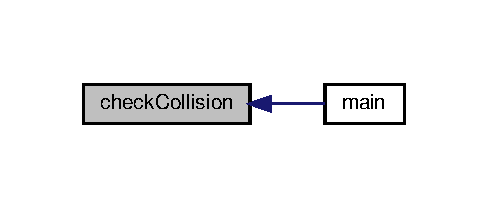
\includegraphics[width=234pt]{container_8c_a7a74c6812adffb8d4419092b999a823b_icgraph}
\end{center}
\end{figure}
\mbox{\Hypertarget{container_8c_a6fe2743b89336db44793a23f4271b75a}\label{container_8c_a6fe2743b89336db44793a23f4271b75a}} 
\index{container.\+c@{container.\+c}!create\+Cross@{create\+Cross}}
\index{create\+Cross@{create\+Cross}!container.\+c@{container.\+c}}
\subsubsection{\texorpdfstring{create\+Cross()}{createCross()}}
{\footnotesize\ttfamily \hyperlink{structcontainer}{container} create\+Cross (\begin{DoxyParamCaption}{ }\end{DoxyParamCaption})}



Definition at line 75 of file container.\+c.



References container\+::data, and init\+Container().



Referenced by random\+Piece().


\begin{DoxyCode}
75                        \{
76     \hyperlink{structcontainer}{container} piece;
77     \hyperlink{container_8c_af20cf8b598b78389dff22b3d176a3727}{initContainer}(5, 5, &piece);
78     piece.\hyperlink{structcontainer_aefae69762fe9c24169e2ca5418a711a1}{data}[2] = 1;
79     piece.\hyperlink{structcontainer_aefae69762fe9c24169e2ca5418a711a1}{data}[7] = 1;
80     piece.\hyperlink{structcontainer_aefae69762fe9c24169e2ca5418a711a1}{data}[10] = 1;
81     piece.\hyperlink{structcontainer_aefae69762fe9c24169e2ca5418a711a1}{data}[11] = 1;
82     piece.\hyperlink{structcontainer_aefae69762fe9c24169e2ca5418a711a1}{data}[12] = 1;
83     piece.\hyperlink{structcontainer_aefae69762fe9c24169e2ca5418a711a1}{data}[13] = 1;
84     piece.\hyperlink{structcontainer_aefae69762fe9c24169e2ca5418a711a1}{data}[14] = 1;
85     piece.\hyperlink{structcontainer_aefae69762fe9c24169e2ca5418a711a1}{data}[17] = 1;
86     piece.\hyperlink{structcontainer_aefae69762fe9c24169e2ca5418a711a1}{data}[22] = 1;
87     piece.\hyperlink{structcontainer_aefae69762fe9c24169e2ca5418a711a1}{data}[24] = 0;
88     \textcolor{keywordflow}{return} piece;
89 \}
\end{DoxyCode}
Here is the call graph for this function\+:
\nopagebreak
\begin{figure}[H]
\begin{center}
\leavevmode
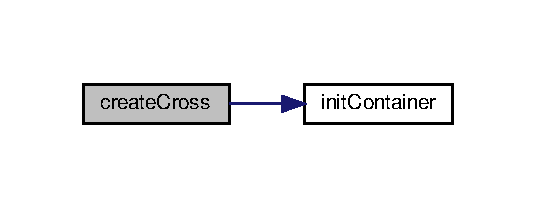
\includegraphics[width=257pt]{container_8c_a6fe2743b89336db44793a23f4271b75a_cgraph}
\end{center}
\end{figure}
Here is the caller graph for this function\+:
\nopagebreak
\begin{figure}[H]
\begin{center}
\leavevmode
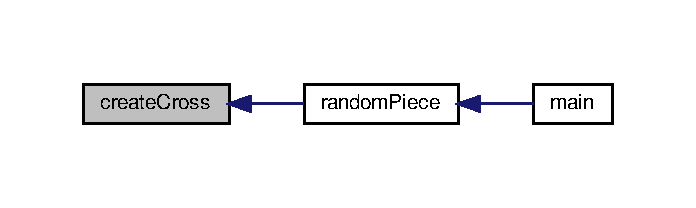
\includegraphics[width=334pt]{container_8c_a6fe2743b89336db44793a23f4271b75a_icgraph}
\end{center}
\end{figure}
\mbox{\Hypertarget{container_8c_a8a2fed74e961c8603aaaacd3ec243111}\label{container_8c_a8a2fed74e961c8603aaaacd3ec243111}} 
\index{container.\+c@{container.\+c}!create\+Dot@{create\+Dot}}
\index{create\+Dot@{create\+Dot}!container.\+c@{container.\+c}}
\subsubsection{\texorpdfstring{create\+Dot()}{createDot()}}
{\footnotesize\ttfamily \hyperlink{structcontainer}{container} create\+Dot (\begin{DoxyParamCaption}{ }\end{DoxyParamCaption})}



Definition at line 91 of file container.\+c.



References container\+::data, and init\+Container().



Referenced by random\+Piece().


\begin{DoxyCode}
91                      \{
92     \hyperlink{structcontainer}{container} piece;
93     \hyperlink{container_8c_af20cf8b598b78389dff22b3d176a3727}{initContainer}(1, 1, &piece);
94     piece.\hyperlink{structcontainer_aefae69762fe9c24169e2ca5418a711a1}{data}[0] = 1;
95     \textcolor{keywordflow}{return} piece;
96 \}
\end{DoxyCode}
Here is the call graph for this function\+:
\nopagebreak
\begin{figure}[H]
\begin{center}
\leavevmode
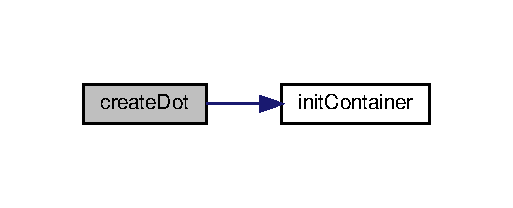
\includegraphics[width=246pt]{container_8c_a8a2fed74e961c8603aaaacd3ec243111_cgraph}
\end{center}
\end{figure}
Here is the caller graph for this function\+:
\nopagebreak
\begin{figure}[H]
\begin{center}
\leavevmode
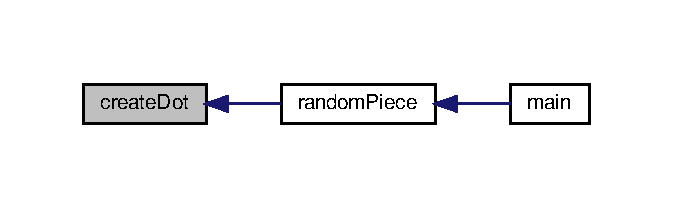
\includegraphics[width=323pt]{container_8c_a8a2fed74e961c8603aaaacd3ec243111_icgraph}
\end{center}
\end{figure}
\mbox{\Hypertarget{container_8c_a7d1d76e4670bb877ca26b4e79db69927}\label{container_8c_a7d1d76e4670bb877ca26b4e79db69927}} 
\index{container.\+c@{container.\+c}!create\+L1@{create\+L1}}
\index{create\+L1@{create\+L1}!container.\+c@{container.\+c}}
\subsubsection{\texorpdfstring{create\+L1()}{createL1()}}
{\footnotesize\ttfamily \hyperlink{structcontainer}{container} create\+L1 (\begin{DoxyParamCaption}{ }\end{DoxyParamCaption})}



Definition at line 55 of file container.\+c.



References container\+::data, and init\+Container().



Referenced by random\+Piece().


\begin{DoxyCode}
55                     \{
56     \hyperlink{structcontainer}{container} piece;
57     \hyperlink{container_8c_af20cf8b598b78389dff22b3d176a3727}{initContainer}(3, 2, &piece);
58     piece.\hyperlink{structcontainer_aefae69762fe9c24169e2ca5418a711a1}{data}[0] = 1;
59     piece.\hyperlink{structcontainer_aefae69762fe9c24169e2ca5418a711a1}{data}[3] = 1;
60     piece.\hyperlink{structcontainer_aefae69762fe9c24169e2ca5418a711a1}{data}[4] = 1;
61     piece.\hyperlink{structcontainer_aefae69762fe9c24169e2ca5418a711a1}{data}[5] = 1;
62     \textcolor{keywordflow}{return} piece;
63 \}
\end{DoxyCode}
Here is the call graph for this function\+:
\nopagebreak
\begin{figure}[H]
\begin{center}
\leavevmode
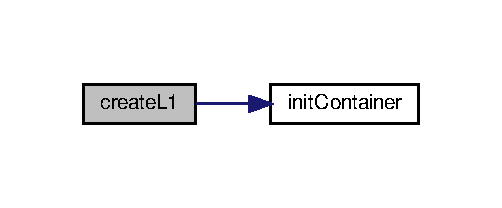
\includegraphics[width=241pt]{container_8c_a7d1d76e4670bb877ca26b4e79db69927_cgraph}
\end{center}
\end{figure}
Here is the caller graph for this function\+:
\nopagebreak
\begin{figure}[H]
\begin{center}
\leavevmode
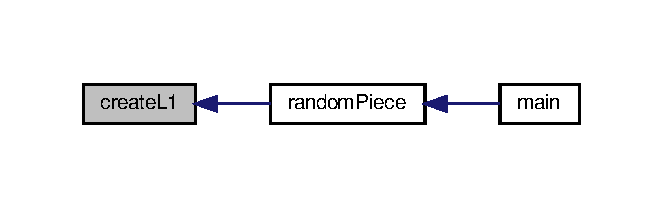
\includegraphics[width=318pt]{container_8c_a7d1d76e4670bb877ca26b4e79db69927_icgraph}
\end{center}
\end{figure}
\mbox{\Hypertarget{container_8c_a4a33c04f7b6aa23f5c9b912bf9c269d7}\label{container_8c_a4a33c04f7b6aa23f5c9b912bf9c269d7}} 
\index{container.\+c@{container.\+c}!create\+L2@{create\+L2}}
\index{create\+L2@{create\+L2}!container.\+c@{container.\+c}}
\subsubsection{\texorpdfstring{create\+L2()}{createL2()}}
{\footnotesize\ttfamily \hyperlink{structcontainer}{container} create\+L2 (\begin{DoxyParamCaption}{ }\end{DoxyParamCaption})}



Definition at line 65 of file container.\+c.



References container\+::data, and init\+Container().



Referenced by random\+Piece().


\begin{DoxyCode}
65                     \{
66     \hyperlink{structcontainer}{container} piece;
67     \hyperlink{container_8c_af20cf8b598b78389dff22b3d176a3727}{initContainer}(3, 2, &piece);
68     piece.\hyperlink{structcontainer_aefae69762fe9c24169e2ca5418a711a1}{data}[2] = 1;
69     piece.\hyperlink{structcontainer_aefae69762fe9c24169e2ca5418a711a1}{data}[3] = 1;
70     piece.\hyperlink{structcontainer_aefae69762fe9c24169e2ca5418a711a1}{data}[4] = 1;
71     piece.\hyperlink{structcontainer_aefae69762fe9c24169e2ca5418a711a1}{data}[5] = 1;
72     \textcolor{keywordflow}{return} piece;
73 \}
\end{DoxyCode}
Here is the call graph for this function\+:
\nopagebreak
\begin{figure}[H]
\begin{center}
\leavevmode
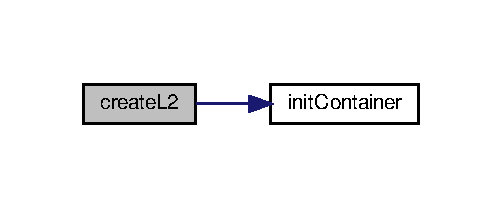
\includegraphics[width=241pt]{container_8c_a4a33c04f7b6aa23f5c9b912bf9c269d7_cgraph}
\end{center}
\end{figure}
Here is the caller graph for this function\+:
\nopagebreak
\begin{figure}[H]
\begin{center}
\leavevmode
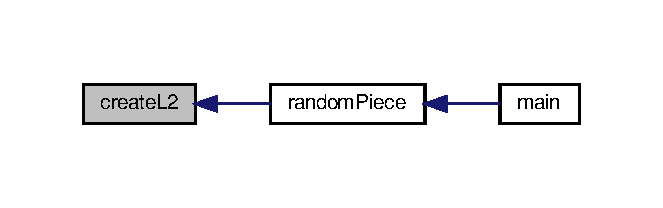
\includegraphics[width=318pt]{container_8c_a4a33c04f7b6aa23f5c9b912bf9c269d7_icgraph}
\end{center}
\end{figure}
\mbox{\Hypertarget{container_8c_ab4a57956d1d813e81c375d37dcd9dd83}\label{container_8c_ab4a57956d1d813e81c375d37dcd9dd83}} 
\index{container.\+c@{container.\+c}!create\+Line@{create\+Line}}
\index{create\+Line@{create\+Line}!container.\+c@{container.\+c}}
\subsubsection{\texorpdfstring{create\+Line()}{createLine()}}
{\footnotesize\ttfamily \hyperlink{structcontainer}{container} create\+Line (\begin{DoxyParamCaption}{ }\end{DoxyParamCaption})}



Definition at line 98 of file container.\+c.



References container\+::data, and init\+Container().



Referenced by random\+Piece().


\begin{DoxyCode}
98                       \{
99     \hyperlink{structcontainer}{container} piece;
100     \hyperlink{container_8c_af20cf8b598b78389dff22b3d176a3727}{initContainer}(1, 2, &piece);
101     piece.\hyperlink{structcontainer_aefae69762fe9c24169e2ca5418a711a1}{data}[0] = 1;
102     piece.\hyperlink{structcontainer_aefae69762fe9c24169e2ca5418a711a1}{data}[1] = 1;
103     \textcolor{keywordflow}{return} piece;
104 \}
\end{DoxyCode}
Here is the call graph for this function\+:
\nopagebreak
\begin{figure}[H]
\begin{center}
\leavevmode
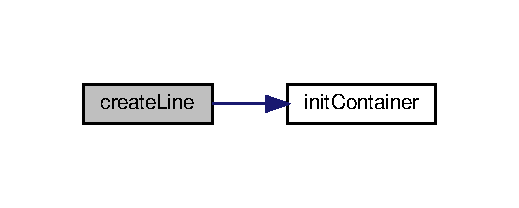
\includegraphics[width=249pt]{container_8c_ab4a57956d1d813e81c375d37dcd9dd83_cgraph}
\end{center}
\end{figure}
Here is the caller graph for this function\+:
\nopagebreak
\begin{figure}[H]
\begin{center}
\leavevmode
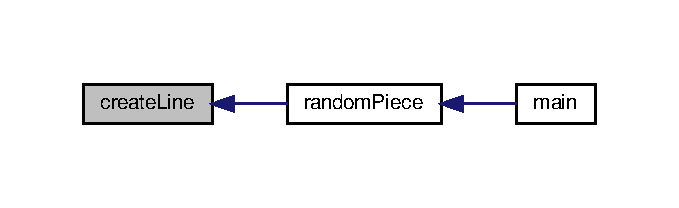
\includegraphics[width=326pt]{container_8c_ab4a57956d1d813e81c375d37dcd9dd83_icgraph}
\end{center}
\end{figure}
\mbox{\Hypertarget{container_8c_acdd60fa36d582876e0c842fadf1816d7}\label{container_8c_acdd60fa36d582876e0c842fadf1816d7}} 
\index{container.\+c@{container.\+c}!createU@{createU}}
\index{createU@{createU}!container.\+c@{container.\+c}}
\subsubsection{\texorpdfstring{create\+U()}{createU()}}
{\footnotesize\ttfamily \hyperlink{structcontainer}{container} createU (\begin{DoxyParamCaption}{ }\end{DoxyParamCaption})}



Definition at line 42 of file container.\+c.



References container\+::data, and init\+Container().



Referenced by random\+Piece().


\begin{DoxyCode}
42                    \{
43     \hyperlink{structcontainer}{container} piece;
44     \hyperlink{container_8c_af20cf8b598b78389dff22b3d176a3727}{initContainer}(3, 3, &piece);
45     piece.\hyperlink{structcontainer_aefae69762fe9c24169e2ca5418a711a1}{data}[0] = 1;
46     piece.\hyperlink{structcontainer_aefae69762fe9c24169e2ca5418a711a1}{data}[2] = 1;
47     piece.\hyperlink{structcontainer_aefae69762fe9c24169e2ca5418a711a1}{data}[3] = 1;
48     piece.\hyperlink{structcontainer_aefae69762fe9c24169e2ca5418a711a1}{data}[5] = 1;
49     piece.\hyperlink{structcontainer_aefae69762fe9c24169e2ca5418a711a1}{data}[6] = 1;
50     piece.\hyperlink{structcontainer_aefae69762fe9c24169e2ca5418a711a1}{data}[7] = 1;
51     piece.\hyperlink{structcontainer_aefae69762fe9c24169e2ca5418a711a1}{data}[8] = 1;
52     \textcolor{keywordflow}{return} piece;
53 \}
\end{DoxyCode}
Here is the call graph for this function\+:
\nopagebreak
\begin{figure}[H]
\begin{center}
\leavevmode
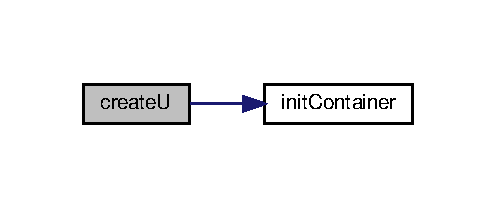
\includegraphics[width=238pt]{container_8c_acdd60fa36d582876e0c842fadf1816d7_cgraph}
\end{center}
\end{figure}
Here is the caller graph for this function\+:
\nopagebreak
\begin{figure}[H]
\begin{center}
\leavevmode
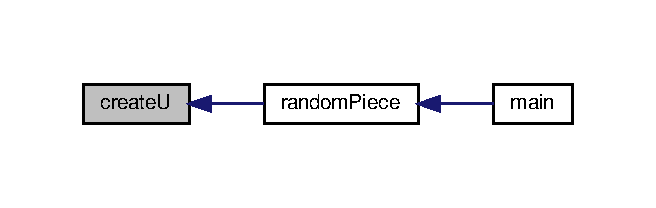
\includegraphics[width=315pt]{container_8c_acdd60fa36d582876e0c842fadf1816d7_icgraph}
\end{center}
\end{figure}
\mbox{\Hypertarget{container_8c_a2a9dbe4ff3be91108eadb428d77debd6}\label{container_8c_a2a9dbe4ff3be91108eadb428d77debd6}} 
\index{container.\+c@{container.\+c}!delete\+Container@{delete\+Container}}
\index{delete\+Container@{delete\+Container}!container.\+c@{container.\+c}}
\subsubsection{\texorpdfstring{delete\+Container()}{deleteContainer()}}
{\footnotesize\ttfamily void delete\+Container (\begin{DoxyParamCaption}\item[{\hyperlink{structcontainer}{container} $\ast$}]{item }\end{DoxyParamCaption})}



Definition at line 106 of file container.\+c.



References container\+::data.


\begin{DoxyCode}
106                                       \{
107     free(item->\hyperlink{structcontainer_aefae69762fe9c24169e2ca5418a711a1}{data});
108 \}
\end{DoxyCode}
\mbox{\Hypertarget{container_8c_af20cf8b598b78389dff22b3d176a3727}\label{container_8c_af20cf8b598b78389dff22b3d176a3727}} 
\index{container.\+c@{container.\+c}!init\+Container@{init\+Container}}
\index{init\+Container@{init\+Container}!container.\+c@{container.\+c}}
\subsubsection{\texorpdfstring{init\+Container()}{initContainer()}}
{\footnotesize\ttfamily void init\+Container (\begin{DoxyParamCaption}\item[{int}]{width,  }\item[{int}]{height,  }\item[{\hyperlink{structcontainer}{container} $\ast$}]{item }\end{DoxyParamCaption})}



Definition at line 3 of file container.\+c.



References container\+::data, container\+::len, and container\+::size.



Referenced by create\+Cross(), create\+Dot(), create\+L1(), create\+L2(), create\+Line(), create\+U(), and main().


\begin{DoxyCode}
3                                                           \{
4     item->\hyperlink{structcontainer_a0069496fb95c879cd33fb79ab726e81a}{len} = width;
5     item->\hyperlink{structcontainer_a1e938d250074e70b9778df1b59121744}{size} = width * height;
6     item->\hyperlink{structcontainer_aefae69762fe9c24169e2ca5418a711a1}{data} = malloc(item->\hyperlink{structcontainer_a1e938d250074e70b9778df1b59121744}{size} * \textcolor{keyword}{sizeof}(\textcolor{keywordtype}{char}));
7     \textcolor{keywordflow}{for} (\textcolor{keywordtype}{int} i = 0; i < item->\hyperlink{structcontainer_a1e938d250074e70b9778df1b59121744}{size}; ++i)
8     \{
9         item->\hyperlink{structcontainer_aefae69762fe9c24169e2ca5418a711a1}{data}[i] = 0;
10     \}
11 \}
\end{DoxyCode}
Here is the caller graph for this function\+:
\nopagebreak
\begin{figure}[H]
\begin{center}
\leavevmode
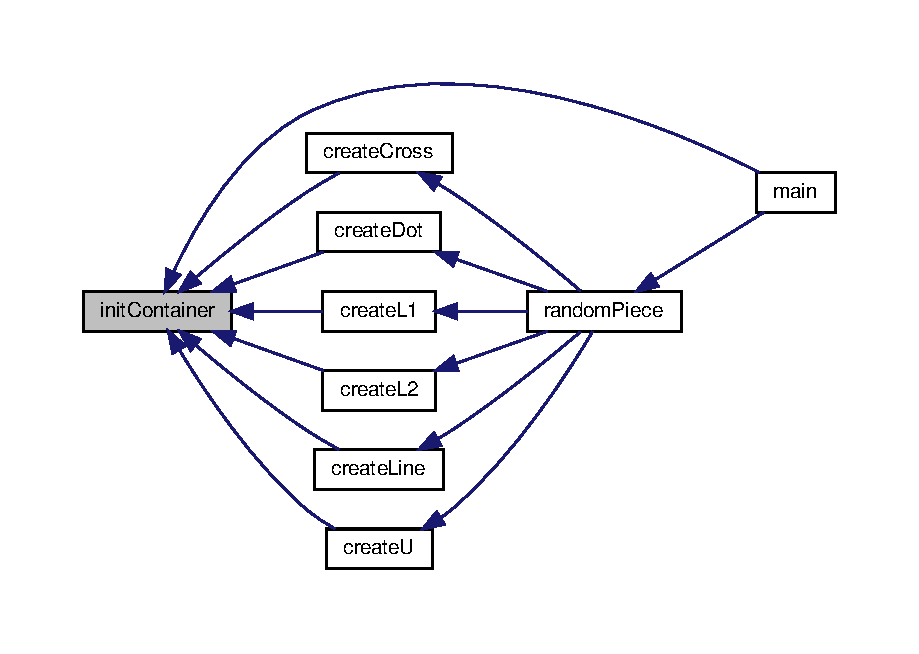
\includegraphics[width=350pt]{container_8c_af20cf8b598b78389dff22b3d176a3727_icgraph}
\end{center}
\end{figure}
\mbox{\Hypertarget{container_8c_a46bfac7d0493d39bd4aad51f270bd0d7}\label{container_8c_a46bfac7d0493d39bd4aad51f270bd0d7}} 
\index{container.\+c@{container.\+c}!place@{place}}
\index{place@{place}!container.\+c@{container.\+c}}
\subsubsection{\texorpdfstring{place()}{place()}}
{\footnotesize\ttfamily void place (\begin{DoxyParamCaption}\item[{\hyperlink{structcontainer}{container} $\ast$}]{grid,  }\item[{\hyperlink{structcontainer}{container} $\ast$}]{piece,  }\item[{int}]{x,  }\item[{int}]{y }\end{DoxyParamCaption})}



Definition at line 124 of file container.\+c.



References container\+::data, container\+::len, and container\+::size.



Referenced by main().


\begin{DoxyCode}
124                                                               \{
125     \textcolor{keywordflow}{for} (\textcolor{keywordtype}{int} i = 0; i < piece->\hyperlink{structcontainer_a1e938d250074e70b9778df1b59121744}{size}/piece->\hyperlink{structcontainer_a0069496fb95c879cd33fb79ab726e81a}{len}; i++) \{
126         \textcolor{keywordflow}{for} (\textcolor{keywordtype}{int} j = 0; j < piece->\hyperlink{structcontainer_a0069496fb95c879cd33fb79ab726e81a}{len}; j++) \{
127             \textcolor{keywordflow}{if} (piece->\hyperlink{structcontainer_aefae69762fe9c24169e2ca5418a711a1}{data}[(i*piece->\hyperlink{structcontainer_a0069496fb95c879cd33fb79ab726e81a}{len})+j] == 1) \{
128                 grid->\hyperlink{structcontainer_aefae69762fe9c24169e2ca5418a711a1}{data}[((i+y)*grid->\hyperlink{structcontainer_a0069496fb95c879cd33fb79ab726e81a}{len})+j+x] = piece->\hyperlink{structcontainer_aefae69762fe9c24169e2ca5418a711a1}{data}[(i*piece->
      \hyperlink{structcontainer_a0069496fb95c879cd33fb79ab726e81a}{len})+j];
129             \}
130         \}
131     \}
132 \}
\end{DoxyCode}
Here is the caller graph for this function\+:
\nopagebreak
\begin{figure}[H]
\begin{center}
\leavevmode
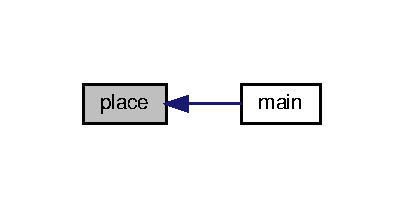
\includegraphics[width=194pt]{container_8c_a46bfac7d0493d39bd4aad51f270bd0d7_icgraph}
\end{center}
\end{figure}
\mbox{\Hypertarget{container_8c_aae1449e449d2f69b52594cccb1dc1e42}\label{container_8c_aae1449e449d2f69b52594cccb1dc1e42}} 
\index{container.\+c@{container.\+c}!random\+Piece@{random\+Piece}}
\index{random\+Piece@{random\+Piece}!container.\+c@{container.\+c}}
\subsubsection{\texorpdfstring{random\+Piece()}{randomPiece()}}
{\footnotesize\ttfamily \hyperlink{structcontainer}{container} random\+Piece (\begin{DoxyParamCaption}{ }\end{DoxyParamCaption})}



Definition at line 13 of file container.\+c.



References create\+Cross(), create\+Dot(), create\+L1(), create\+L2(), create\+Line(), and create\+U().



Referenced by main().


\begin{DoxyCode}
13                        \{
14     \hyperlink{structcontainer}{container} piece;
15     srand(time(NULL));
16     \textcolor{keywordtype}{int} random = rand() % 6;
17     \textcolor{keywordflow}{switch} (random)\{
18         \textcolor{keywordflow}{case} 0 :
19             piece = \hyperlink{container_8c_acdd60fa36d582876e0c842fadf1816d7}{createU}();
20             \textcolor{keywordflow}{return} piece;
21         \textcolor{keywordflow}{case} 1 :
22             piece = \hyperlink{container_8c_a7d1d76e4670bb877ca26b4e79db69927}{createL1}();
23             \textcolor{keywordflow}{return} piece;
24         \textcolor{keywordflow}{case} 2 :
25             piece = \hyperlink{container_8c_a4a33c04f7b6aa23f5c9b912bf9c269d7}{createL2}();
26             \textcolor{keywordflow}{return} piece;
27         \textcolor{keywordflow}{case} 3 :
28             piece = \hyperlink{container_8c_a6fe2743b89336db44793a23f4271b75a}{createCross}();
29             \textcolor{keywordflow}{return} piece;
30         \textcolor{keywordflow}{case} 4:
31             piece = \hyperlink{container_8c_a8a2fed74e961c8603aaaacd3ec243111}{createDot}();
32             \textcolor{keywordflow}{return} piece;
33         \textcolor{keywordflow}{case} 5 :
34             piece = \hyperlink{container_8c_ab4a57956d1d813e81c375d37dcd9dd83}{createLine}();
35             \textcolor{keywordflow}{return} piece;
36         default :
37             printf(\textcolor{stringliteral}{"Error : could not generate cooresponding piece for int : %d \(\backslash\)n"}, random);
38             exit(0);
39     \}
40 \}
\end{DoxyCode}
Here is the call graph for this function\+:
\nopagebreak
\begin{figure}[H]
\begin{center}
\leavevmode
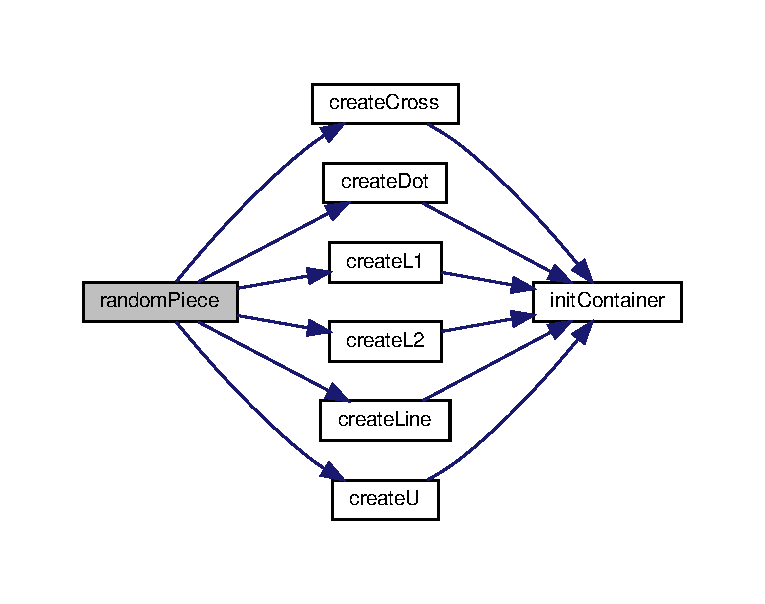
\includegraphics[width=350pt]{container_8c_aae1449e449d2f69b52594cccb1dc1e42_cgraph}
\end{center}
\end{figure}
Here is the caller graph for this function\+:
\nopagebreak
\begin{figure}[H]
\begin{center}
\leavevmode
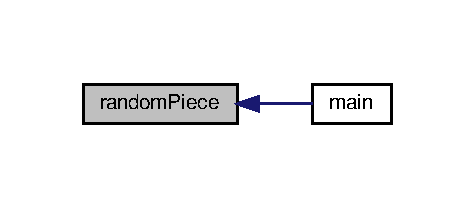
\includegraphics[width=228pt]{container_8c_aae1449e449d2f69b52594cccb1dc1e42_icgraph}
\end{center}
\end{figure}

\hypertarget{head_8h}{}\section{head.\+h File Reference}
\label{head_8h}\index{head.\+h@{head.\+h}}
{\ttfamily \#include $<$time.\+h$>$}\newline
{\ttfamily \#include $<$stdlib.\+h$>$}\newline
{\ttfamily \#include $<$stdio.\+h$>$}\newline
{\ttfamily \#include $<$string.\+h$>$}\newline
Include dependency graph for head.\+h\+:
% FIG 0
This graph shows which files directly or indirectly include this file\+:
% FIG 1
\subsection*{Data Structures}
\begin{DoxyCompactItemize}
\item 
struct \hyperlink{structcontainer}{container}
\end{DoxyCompactItemize}
\subsection*{Macros}
\begin{DoxyCompactItemize}
\item 
\#define \hyperlink{head_8h_a241aeeb764887ae5e3de58b98f04b16d}{W\+I\+D\+TH}~20
\item 
\#define \hyperlink{head_8h_aed89bd71aee8be823e8a20ec4e093c1e}{H\+E\+I\+G\+HT}~25
\end{DoxyCompactItemize}
\subsection*{Functions}
\begin{DoxyCompactItemize}
\item 
int $\ast$ \hyperlink{head_8h_af9526652ed9443df3955c6cac0fe12c7}{detect\+Row} (\hyperlink{structcontainer}{container} $\ast$grid)
\item 
char \hyperlink{head_8h_a35c79938c8ccc4683d509620aa6e15af}{full\+Row} (\hyperlink{structcontainer}{container} $\ast$grid, int index)
\item 
void \hyperlink{head_8h_a1b4ff27dd8eca8ec63460b424310d541}{delete\+Row} (\hyperlink{structcontainer}{container} $\ast$grid, int $\ast$index\+List)
\item 
int $\ast$ \hyperlink{head_8h_a0e35a2936fc69af30890ce30a082b594}{detect\+Col} (\hyperlink{structcontainer}{container} $\ast$grid)
\item 
char \hyperlink{head_8h_aebb74ac9ba3f8c734beba4617a6bf439}{full\+Col} (\hyperlink{structcontainer}{container} $\ast$grid, int index)
\item 
void \hyperlink{head_8h_a7bf753ec2f6d5d89d3cfbce8d704428f}{delete\+Col} (\hyperlink{structcontainer}{container} $\ast$grid, int $\ast$index\+List)
\item 
void \hyperlink{head_8h_afdd0072ee83eaeca8b99941e73bf2c8e}{gravity} (\hyperlink{structcontainer}{container} $\ast$grid, int $\ast$index\+\_\+list\+\_\+line, int $\ast$index\+\_\+list\+\_\+col)
\item 
void \hyperlink{head_8h_aca3f584034ddadfcf89951a1bf10f45c}{update} (\hyperlink{structcontainer}{container} $\ast$grid)
\item 
void \hyperlink{head_8h_af20cf8b598b78389dff22b3d176a3727}{init\+Container} (int width, int height, \hyperlink{structcontainer}{container} $\ast$item)
\item 
\hyperlink{structcontainer}{container} \hyperlink{head_8h_aae1449e449d2f69b52594cccb1dc1e42}{random\+Piece} ()
\item 
\hyperlink{structcontainer}{container} \hyperlink{head_8h_acdd60fa36d582876e0c842fadf1816d7}{createU} ()
\item 
\hyperlink{structcontainer}{container} \hyperlink{head_8h_a7d1d76e4670bb877ca26b4e79db69927}{create\+L1} ()
\item 
\hyperlink{structcontainer}{container} \hyperlink{head_8h_a4a33c04f7b6aa23f5c9b912bf9c269d7}{create\+L2} ()
\item 
\hyperlink{structcontainer}{container} \hyperlink{head_8h_a6fe2743b89336db44793a23f4271b75a}{create\+Cross} ()
\item 
\hyperlink{structcontainer}{container} \hyperlink{head_8h_a8a2fed74e961c8603aaaacd3ec243111}{create\+Dot} ()
\item 
\hyperlink{structcontainer}{container} \hyperlink{head_8h_ab4a57956d1d813e81c375d37dcd9dd83}{create\+Line} ()
\item 
void \hyperlink{head_8h_a2a9dbe4ff3be91108eadb428d77debd6}{delete\+Container} (\hyperlink{structcontainer}{container} $\ast$item)
\item 
int \hyperlink{head_8h_a7a74c6812adffb8d4419092b999a823b}{check\+Collision} (\hyperlink{structcontainer}{container} $\ast$grid, \hyperlink{structcontainer}{container} $\ast$piece, int x, int y)
\item 
void \hyperlink{head_8h_a46bfac7d0493d39bd4aad51f270bd0d7}{place} (\hyperlink{structcontainer}{container} $\ast$grid, \hyperlink{structcontainer}{container} $\ast$piece, int x, int y)
\item 
void \hyperlink{head_8h_ac2b3cb6c7ec0748f0c4c1a46e0997d70}{display} (\hyperlink{structcontainer}{container} $\ast$grid)
\item 
void \hyperlink{head_8h_a44fa0cbfa7fc79473c8ac9ca3b198f5a}{rotate\+\_\+90} (\hyperlink{structcontainer}{container} $\ast$piece)
\item 
void \hyperlink{head_8h_afbdf40ca68538464d0df29d9b2a77366}{rotate\+\_\+180} (\hyperlink{structcontainer}{container} $\ast$piece)
\end{DoxyCompactItemize}


\subsection{Macro Definition Documentation}
\mbox{\Hypertarget{head_8h_aed89bd71aee8be823e8a20ec4e093c1e}\label{head_8h_aed89bd71aee8be823e8a20ec4e093c1e}} 
\index{head.\+h@{head.\+h}!H\+E\+I\+G\+HT@{H\+E\+I\+G\+HT}}
\index{H\+E\+I\+G\+HT@{H\+E\+I\+G\+HT}!head.\+h@{head.\+h}}
\subsubsection{\texorpdfstring{H\+E\+I\+G\+HT}{HEIGHT}}
{\footnotesize\ttfamily \#define H\+E\+I\+G\+HT~25}



Definition at line 12 of file head.\+h.



Referenced by main().

\mbox{\Hypertarget{head_8h_a241aeeb764887ae5e3de58b98f04b16d}\label{head_8h_a241aeeb764887ae5e3de58b98f04b16d}} 
\index{head.\+h@{head.\+h}!W\+I\+D\+TH@{W\+I\+D\+TH}}
\index{W\+I\+D\+TH@{W\+I\+D\+TH}!head.\+h@{head.\+h}}
\subsubsection{\texorpdfstring{W\+I\+D\+TH}{WIDTH}}
{\footnotesize\ttfamily \#define W\+I\+D\+TH~20}



Definition at line 11 of file head.\+h.



Referenced by main().



\subsection{Function Documentation}
\mbox{\Hypertarget{head_8h_a7a74c6812adffb8d4419092b999a823b}\label{head_8h_a7a74c6812adffb8d4419092b999a823b}} 
\index{head.\+h@{head.\+h}!check\+Collision@{check\+Collision}}
\index{check\+Collision@{check\+Collision}!head.\+h@{head.\+h}}
\subsubsection{\texorpdfstring{check\+Collision()}{checkCollision()}}
{\footnotesize\ttfamily int check\+Collision (\begin{DoxyParamCaption}\item[{\hyperlink{structcontainer}{container} $\ast$}]{grid,  }\item[{\hyperlink{structcontainer}{container} $\ast$}]{piece,  }\item[{int}]{x,  }\item[{int}]{y }\end{DoxyParamCaption})}



Definition at line 110 of file container.\+c.



References container\+::data, container\+::len, and container\+::size.



Referenced by main().


\begin{DoxyCode}
110                                                                      \{
111     \textcolor{keywordflow}{for} (\textcolor{keywordtype}{int} i = 0; i < piece->\hyperlink{structcontainer_a1e938d250074e70b9778df1b59121744}{size}/piece->\hyperlink{structcontainer_a0069496fb95c879cd33fb79ab726e81a}{len}; i++) \{
112         \textcolor{keywordflow}{for} (\textcolor{keywordtype}{int} j = 0; j < piece->\hyperlink{structcontainer_a0069496fb95c879cd33fb79ab726e81a}{len}; j++) \{
113             \textcolor{keywordflow}{if} (i+y < 0 || i+y >= (grid->\hyperlink{structcontainer_a1e938d250074e70b9778df1b59121744}{size}/grid->\hyperlink{structcontainer_a0069496fb95c879cd33fb79ab726e81a}{len}) || j+x < 0 || j+x >= grid->
      \hyperlink{structcontainer_a0069496fb95c879cd33fb79ab726e81a}{len}) \{
114                 \textcolor{keywordflow}{return} 1;
115             \}
116             \textcolor{keywordflow}{if} (grid->\hyperlink{structcontainer_aefae69762fe9c24169e2ca5418a711a1}{data}[((i+y)*grid->\hyperlink{structcontainer_a0069496fb95c879cd33fb79ab726e81a}{len})+j+x] && piece->\hyperlink{structcontainer_aefae69762fe9c24169e2ca5418a711a1}{data}[(i*piece->
      \hyperlink{structcontainer_a0069496fb95c879cd33fb79ab726e81a}{len})+j]) \{
117                 \textcolor{keywordflow}{return} 1;
118             \}
119         \}
120     \}
121     \textcolor{keywordflow}{return} 0;
122 \}
\end{DoxyCode}
Here is the caller graph for this function\+:
% FIG 2
\mbox{\Hypertarget{head_8h_a6fe2743b89336db44793a23f4271b75a}\label{head_8h_a6fe2743b89336db44793a23f4271b75a}} 
\index{head.\+h@{head.\+h}!create\+Cross@{create\+Cross}}
\index{create\+Cross@{create\+Cross}!head.\+h@{head.\+h}}
\subsubsection{\texorpdfstring{create\+Cross()}{createCross()}}
{\footnotesize\ttfamily \hyperlink{structcontainer}{container} create\+Cross (\begin{DoxyParamCaption}{ }\end{DoxyParamCaption})}



Definition at line 75 of file container.\+c.



References container\+::data, and init\+Container().



Referenced by random\+Piece().


\begin{DoxyCode}
75                        \{
76     \hyperlink{structcontainer}{container} piece;
77     \hyperlink{container_8c_af20cf8b598b78389dff22b3d176a3727}{initContainer}(5, 5, &piece);
78     piece.\hyperlink{structcontainer_aefae69762fe9c24169e2ca5418a711a1}{data}[2] = 1;
79     piece.\hyperlink{structcontainer_aefae69762fe9c24169e2ca5418a711a1}{data}[7] = 1;
80     piece.\hyperlink{structcontainer_aefae69762fe9c24169e2ca5418a711a1}{data}[10] = 1;
81     piece.\hyperlink{structcontainer_aefae69762fe9c24169e2ca5418a711a1}{data}[11] = 1;
82     piece.\hyperlink{structcontainer_aefae69762fe9c24169e2ca5418a711a1}{data}[12] = 1;
83     piece.\hyperlink{structcontainer_aefae69762fe9c24169e2ca5418a711a1}{data}[13] = 1;
84     piece.\hyperlink{structcontainer_aefae69762fe9c24169e2ca5418a711a1}{data}[14] = 1;
85     piece.\hyperlink{structcontainer_aefae69762fe9c24169e2ca5418a711a1}{data}[17] = 1;
86     piece.\hyperlink{structcontainer_aefae69762fe9c24169e2ca5418a711a1}{data}[22] = 1;
87     piece.\hyperlink{structcontainer_aefae69762fe9c24169e2ca5418a711a1}{data}[24] = 0;
88     \textcolor{keywordflow}{return} piece;
89 \}
\end{DoxyCode}
Here is the call graph for this function\+:
% FIG 3
Here is the caller graph for this function\+:
% FIG 4
\mbox{\Hypertarget{head_8h_a8a2fed74e961c8603aaaacd3ec243111}\label{head_8h_a8a2fed74e961c8603aaaacd3ec243111}} 
\index{head.\+h@{head.\+h}!create\+Dot@{create\+Dot}}
\index{create\+Dot@{create\+Dot}!head.\+h@{head.\+h}}
\subsubsection{\texorpdfstring{create\+Dot()}{createDot()}}
{\footnotesize\ttfamily \hyperlink{structcontainer}{container} create\+Dot (\begin{DoxyParamCaption}{ }\end{DoxyParamCaption})}



Definition at line 91 of file container.\+c.



References container\+::data, and init\+Container().



Referenced by random\+Piece().


\begin{DoxyCode}
91                      \{
92     \hyperlink{structcontainer}{container} piece;
93     \hyperlink{container_8c_af20cf8b598b78389dff22b3d176a3727}{initContainer}(1, 1, &piece);
94     piece.\hyperlink{structcontainer_aefae69762fe9c24169e2ca5418a711a1}{data}[0] = 1;
95     \textcolor{keywordflow}{return} piece;
96 \}
\end{DoxyCode}
Here is the call graph for this function\+:
% FIG 5
Here is the caller graph for this function\+:
% FIG 6
\mbox{\Hypertarget{head_8h_a7d1d76e4670bb877ca26b4e79db69927}\label{head_8h_a7d1d76e4670bb877ca26b4e79db69927}} 
\index{head.\+h@{head.\+h}!create\+L1@{create\+L1}}
\index{create\+L1@{create\+L1}!head.\+h@{head.\+h}}
\subsubsection{\texorpdfstring{create\+L1()}{createL1()}}
{\footnotesize\ttfamily \hyperlink{structcontainer}{container} create\+L1 (\begin{DoxyParamCaption}{ }\end{DoxyParamCaption})}



Definition at line 55 of file container.\+c.



References container\+::data, and init\+Container().



Referenced by random\+Piece().


\begin{DoxyCode}
55                     \{
56     \hyperlink{structcontainer}{container} piece;
57     \hyperlink{container_8c_af20cf8b598b78389dff22b3d176a3727}{initContainer}(3, 2, &piece);
58     piece.\hyperlink{structcontainer_aefae69762fe9c24169e2ca5418a711a1}{data}[0] = 1;
59     piece.\hyperlink{structcontainer_aefae69762fe9c24169e2ca5418a711a1}{data}[3] = 1;
60     piece.\hyperlink{structcontainer_aefae69762fe9c24169e2ca5418a711a1}{data}[4] = 1;
61     piece.\hyperlink{structcontainer_aefae69762fe9c24169e2ca5418a711a1}{data}[5] = 1;
62     \textcolor{keywordflow}{return} piece;
63 \}
\end{DoxyCode}
Here is the call graph for this function\+:
% FIG 7
Here is the caller graph for this function\+:
% FIG 8
\mbox{\Hypertarget{head_8h_a4a33c04f7b6aa23f5c9b912bf9c269d7}\label{head_8h_a4a33c04f7b6aa23f5c9b912bf9c269d7}} 
\index{head.\+h@{head.\+h}!create\+L2@{create\+L2}}
\index{create\+L2@{create\+L2}!head.\+h@{head.\+h}}
\subsubsection{\texorpdfstring{create\+L2()}{createL2()}}
{\footnotesize\ttfamily \hyperlink{structcontainer}{container} create\+L2 (\begin{DoxyParamCaption}{ }\end{DoxyParamCaption})}



Definition at line 65 of file container.\+c.



References container\+::data, and init\+Container().



Referenced by random\+Piece().


\begin{DoxyCode}
65                     \{
66     \hyperlink{structcontainer}{container} piece;
67     \hyperlink{container_8c_af20cf8b598b78389dff22b3d176a3727}{initContainer}(3, 2, &piece);
68     piece.\hyperlink{structcontainer_aefae69762fe9c24169e2ca5418a711a1}{data}[2] = 1;
69     piece.\hyperlink{structcontainer_aefae69762fe9c24169e2ca5418a711a1}{data}[3] = 1;
70     piece.\hyperlink{structcontainer_aefae69762fe9c24169e2ca5418a711a1}{data}[4] = 1;
71     piece.\hyperlink{structcontainer_aefae69762fe9c24169e2ca5418a711a1}{data}[5] = 1;
72     \textcolor{keywordflow}{return} piece;
73 \}
\end{DoxyCode}
Here is the call graph for this function\+:
% FIG 9
Here is the caller graph for this function\+:
% FIG 10
\mbox{\Hypertarget{head_8h_ab4a57956d1d813e81c375d37dcd9dd83}\label{head_8h_ab4a57956d1d813e81c375d37dcd9dd83}} 
\index{head.\+h@{head.\+h}!create\+Line@{create\+Line}}
\index{create\+Line@{create\+Line}!head.\+h@{head.\+h}}
\subsubsection{\texorpdfstring{create\+Line()}{createLine()}}
{\footnotesize\ttfamily \hyperlink{structcontainer}{container} create\+Line (\begin{DoxyParamCaption}{ }\end{DoxyParamCaption})}



Definition at line 98 of file container.\+c.



References container\+::data, and init\+Container().



Referenced by random\+Piece().


\begin{DoxyCode}
98                       \{
99     \hyperlink{structcontainer}{container} piece;
100     \hyperlink{container_8c_af20cf8b598b78389dff22b3d176a3727}{initContainer}(1, 2, &piece);
101     piece.\hyperlink{structcontainer_aefae69762fe9c24169e2ca5418a711a1}{data}[0] = 1;
102     piece.\hyperlink{structcontainer_aefae69762fe9c24169e2ca5418a711a1}{data}[1] = 1;
103     \textcolor{keywordflow}{return} piece;
104 \}
\end{DoxyCode}
Here is the call graph for this function\+:
% FIG 11
Here is the caller graph for this function\+:
% FIG 12
\mbox{\Hypertarget{head_8h_acdd60fa36d582876e0c842fadf1816d7}\label{head_8h_acdd60fa36d582876e0c842fadf1816d7}} 
\index{head.\+h@{head.\+h}!createU@{createU}}
\index{createU@{createU}!head.\+h@{head.\+h}}
\subsubsection{\texorpdfstring{create\+U()}{createU()}}
{\footnotesize\ttfamily \hyperlink{structcontainer}{container} createU (\begin{DoxyParamCaption}{ }\end{DoxyParamCaption})}



Definition at line 42 of file container.\+c.



References container\+::data, and init\+Container().



Referenced by random\+Piece().


\begin{DoxyCode}
42                    \{
43     \hyperlink{structcontainer}{container} piece;
44     \hyperlink{container_8c_af20cf8b598b78389dff22b3d176a3727}{initContainer}(3, 3, &piece);
45     piece.\hyperlink{structcontainer_aefae69762fe9c24169e2ca5418a711a1}{data}[0] = 1;
46     piece.\hyperlink{structcontainer_aefae69762fe9c24169e2ca5418a711a1}{data}[2] = 1;
47     piece.\hyperlink{structcontainer_aefae69762fe9c24169e2ca5418a711a1}{data}[3] = 1;
48     piece.\hyperlink{structcontainer_aefae69762fe9c24169e2ca5418a711a1}{data}[5] = 1;
49     piece.\hyperlink{structcontainer_aefae69762fe9c24169e2ca5418a711a1}{data}[6] = 1;
50     piece.\hyperlink{structcontainer_aefae69762fe9c24169e2ca5418a711a1}{data}[7] = 1;
51     piece.\hyperlink{structcontainer_aefae69762fe9c24169e2ca5418a711a1}{data}[8] = 1;
52     \textcolor{keywordflow}{return} piece;
53 \}
\end{DoxyCode}
Here is the call graph for this function\+:
% FIG 13
Here is the caller graph for this function\+:
% FIG 14
\mbox{\Hypertarget{head_8h_a7bf753ec2f6d5d89d3cfbce8d704428f}\label{head_8h_a7bf753ec2f6d5d89d3cfbce8d704428f}} 
\index{head.\+h@{head.\+h}!delete\+Col@{delete\+Col}}
\index{delete\+Col@{delete\+Col}!head.\+h@{head.\+h}}
\subsubsection{\texorpdfstring{delete\+Col()}{deleteCol()}}
{\footnotesize\ttfamily void delete\+Col (\begin{DoxyParamCaption}\item[{\hyperlink{structcontainer}{container} $\ast$}]{grid,  }\item[{int $\ast$}]{index\+List }\end{DoxyParamCaption})}



Definition at line 108 of file update.\+c.



References container\+::data, container\+::len, and container\+::size.



Referenced by update().


\begin{DoxyCode}
108                                                 \{
109 
110     \textcolor{keywordtype}{int} actual, max\_len, max\_size, max\_size1, i, j;
111     \textcolor{keywordtype}{char} *save\_data;
112 
113     \textcolor{comment}{//Sauvegarde}
114     save\_data = grid->\hyperlink{structcontainer_aefae69762fe9c24169e2ca5418a711a1}{data};
115     max\_len = grid->\hyperlink{structcontainer_a0069496fb95c879cd33fb79ab726e81a}{len};
116     max\_size1 = grid->\hyperlink{structcontainer_a1e938d250074e70b9778df1b59121744}{size};
117 
118     max\_size = index\_list[0];
119 
120     \textcolor{keywordflow}{for}(i=1; i<max\_size; ++i)\{
121         actual = index\_list[i];
122         \textcolor{keywordflow}{for}(j=actual; j< max\_size1; j += max\_len)\{
123             save\_data[j] = 0;
124         \}
125     \}
126 
127 \}
\end{DoxyCode}
Here is the caller graph for this function\+:
% FIG 15
\mbox{\Hypertarget{head_8h_a2a9dbe4ff3be91108eadb428d77debd6}\label{head_8h_a2a9dbe4ff3be91108eadb428d77debd6}} 
\index{head.\+h@{head.\+h}!delete\+Container@{delete\+Container}}
\index{delete\+Container@{delete\+Container}!head.\+h@{head.\+h}}
\subsubsection{\texorpdfstring{delete\+Container()}{deleteContainer()}}
{\footnotesize\ttfamily void delete\+Container (\begin{DoxyParamCaption}\item[{\hyperlink{structcontainer}{container} $\ast$}]{item }\end{DoxyParamCaption})}



Definition at line 106 of file container.\+c.



References container\+::data.


\begin{DoxyCode}
106                                       \{
107     free(item->\hyperlink{structcontainer_aefae69762fe9c24169e2ca5418a711a1}{data});
108 \}
\end{DoxyCode}
\mbox{\Hypertarget{head_8h_a1b4ff27dd8eca8ec63460b424310d541}\label{head_8h_a1b4ff27dd8eca8ec63460b424310d541}} 
\index{head.\+h@{head.\+h}!delete\+Row@{delete\+Row}}
\index{delete\+Row@{delete\+Row}!head.\+h@{head.\+h}}
\subsubsection{\texorpdfstring{delete\+Row()}{deleteRow()}}
{\footnotesize\ttfamily void delete\+Row (\begin{DoxyParamCaption}\item[{\hyperlink{structcontainer}{container} $\ast$}]{grid,  }\item[{int $\ast$}]{index\+List }\end{DoxyParamCaption})}



Definition at line 44 of file update.\+c.



References container\+::data, and container\+::len.



Referenced by update().


\begin{DoxyCode}
44                                                 \{
45 
46     \textcolor{keywordtype}{int} actual, max\_len, max\_size, i, j;
47     \textcolor{keywordtype}{char} *save\_data;
48 
49     \textcolor{comment}{//Sauvegarde}
50     save\_data = grid->\hyperlink{structcontainer_aefae69762fe9c24169e2ca5418a711a1}{data};
51     max\_len = grid->\hyperlink{structcontainer_a0069496fb95c879cd33fb79ab726e81a}{len};
52 
53     max\_size = index\_list[0];
54     \textcolor{keywordflow}{for}(i=1; i<max\_size; ++i)\{
55         actual = index\_list[i];
56         \textcolor{keywordflow}{for}(j=actual; j< actual + max\_len; ++j)\{
57             save\_data[j] = 0;
58         \}
59     \}
60 
61 \}
\end{DoxyCode}
Here is the caller graph for this function\+:
% FIG 16
\mbox{\Hypertarget{head_8h_a0e35a2936fc69af30890ce30a082b594}\label{head_8h_a0e35a2936fc69af30890ce30a082b594}} 
\index{head.\+h@{head.\+h}!detect\+Col@{detect\+Col}}
\index{detect\+Col@{detect\+Col}!head.\+h@{head.\+h}}
\subsubsection{\texorpdfstring{detect\+Col()}{detectCol()}}
{\footnotesize\ttfamily int$\ast$ detect\+Col (\begin{DoxyParamCaption}\item[{\hyperlink{structcontainer}{container} $\ast$}]{grid }\end{DoxyParamCaption})}



Definition at line 66 of file update.\+c.



References full\+Col(), and container\+::len.



Referenced by update().


\begin{DoxyCode}
66                                \{
67 
68     \textcolor{keywordtype}{int} *index, actual, max\_len, i;
69 
70     \textcolor{comment}{//save}
71     max\_len = grid->\hyperlink{structcontainer_a0069496fb95c879cd33fb79ab726e81a}{len};
72 
73     \textcolor{comment}{//Index}
74     actual = 1;
75     index = malloc((max\_len+1)*\textcolor{keyword}{sizeof}(\textcolor{keywordtype}{int}));
76 
77     \textcolor{keywordflow}{for}(i=0; i<max\_len; ++i)\{
78         \textcolor{keywordflow}{if}(\hyperlink{update_8c_aebb74ac9ba3f8c734beba4617a6bf439}{fullCol}(grid, i))\{
79             index[actual] = i;
80             ++actual;
81         \}
82     \}
83 
84     index[0] = actual;
85 
86     \textcolor{keywordflow}{return} realloc(index, actual);
87 \}
\end{DoxyCode}
Here is the call graph for this function\+:
% FIG 17
Here is the caller graph for this function\+:
% FIG 18
\mbox{\Hypertarget{head_8h_af9526652ed9443df3955c6cac0fe12c7}\label{head_8h_af9526652ed9443df3955c6cac0fe12c7}} 
\index{head.\+h@{head.\+h}!detect\+Row@{detect\+Row}}
\index{detect\+Row@{detect\+Row}!head.\+h@{head.\+h}}
\subsubsection{\texorpdfstring{detect\+Row()}{detectRow()}}
{\footnotesize\ttfamily int$\ast$ detect\+Row (\begin{DoxyParamCaption}\item[{\hyperlink{structcontainer}{container} $\ast$}]{grid }\end{DoxyParamCaption})}



Definition at line 4 of file update.\+c.



References full\+Row(), container\+::len, and container\+::size.



Referenced by update().


\begin{DoxyCode}
4                                \{
5 
6     \textcolor{keywordtype}{int} *index, actual, max\_len, max\_size, i;
7 
8     \textcolor{comment}{//Sauvegarde}
9     max\_len = grid->\hyperlink{structcontainer_a0069496fb95c879cd33fb79ab726e81a}{len};
10     max\_size = grid->\hyperlink{structcontainer_a1e938d250074e70b9778df1b59121744}{size};
11 
12     \textcolor{comment}{//Index}
13     actual = 1;
14     index = malloc((max\_size/max\_len + 1)*\textcolor{keyword}{sizeof}(\textcolor{keywordtype}{int}));
15 
16     \textcolor{keywordflow}{for}(i=0; i<max\_size; i += max\_len)\{
17         \textcolor{keywordflow}{if}(\hyperlink{update_8c_a35c79938c8ccc4683d509620aa6e15af}{fullRow}(grid, i))\{
18             index[actual] = i;
19             ++actual;
20         \}
21     \}
22     index[0] = actual;
23 
24     \textcolor{keywordflow}{return} realloc(index, actual);
25 \}
\end{DoxyCode}
Here is the call graph for this function\+:
% FIG 19
Here is the caller graph for this function\+:
% FIG 20
\mbox{\Hypertarget{head_8h_ac2b3cb6c7ec0748f0c4c1a46e0997d70}\label{head_8h_ac2b3cb6c7ec0748f0c4c1a46e0997d70}} 
\index{head.\+h@{head.\+h}!display@{display}}
\index{display@{display}!head.\+h@{head.\+h}}
\subsubsection{\texorpdfstring{display()}{display()}}
{\footnotesize\ttfamily void display (\begin{DoxyParamCaption}\item[{\hyperlink{structcontainer}{container} $\ast$}]{grid }\end{DoxyParamCaption})}



Definition at line 3 of file user.\+c.



References container\+::data, container\+::len, and container\+::size.



Referenced by main().


\begin{DoxyCode}
3                              \{
4     \textcolor{keywordtype}{char} *toShow = \textcolor{stringliteral}{"36m"};
5     \textcolor{keywordtype}{int} i;
6 
7     \textcolor{keywordflow}{for} (i = 0; i < grid->\hyperlink{structcontainer_a0069496fb95c879cd33fb79ab726e81a}{len}+2; i++) \{
8         printf(\textcolor{stringliteral}{"-"});
9     \}
10     printf(\textcolor{stringliteral}{"\(\backslash\)n|"});
11 
12     \textcolor{keywordflow}{for} (i = 0; i < grid->\hyperlink{structcontainer_a1e938d250074e70b9778df1b59121744}{size}; i++) \{
13         \textcolor{keywordflow}{if} (i % grid->\hyperlink{structcontainer_a0069496fb95c879cd33fb79ab726e81a}{len} == 0 && i != 0) \{
14             printf(\textcolor{stringliteral}{"|%d\(\backslash\)n|"}, (i/grid->\hyperlink{structcontainer_a0069496fb95c879cd33fb79ab726e81a}{len})-1);  \textcolor{comment}{// Erreur ! Affichage de 23 puis 25 dans les deux
       dernières lignes de la zone de jeu, et même phénomène pour la preview pièce}
15         \}
16 
17         \textcolor{keywordflow}{switch} (grid->\hyperlink{structcontainer_aefae69762fe9c24169e2ca5418a711a1}{data}[i]) \{
18             \textcolor{keywordflow}{case} 2:
19                 toShow = \textcolor{stringliteral}{"31m"};
20                 \textcolor{keywordflow}{break};
21         \}
22 
23         \textcolor{keywordflow}{if} (grid->\hyperlink{structcontainer_aefae69762fe9c24169e2ca5418a711a1}{data}[i] > 0)\{
24             printf(\textcolor{stringliteral}{"\(\backslash\)033[%sX"}, toShow);
25         \}\textcolor{keywordflow}{else}\{
26             printf(\textcolor{stringliteral}{" "});
27         \}
28     \}
29     printf(\textcolor{stringliteral}{"|%d\(\backslash\)n"},i/grid->\hyperlink{structcontainer_a0069496fb95c879cd33fb79ab726e81a}{len}-1);
30     \textcolor{keywordflow}{for} (i = 0; i < grid->\hyperlink{structcontainer_a0069496fb95c879cd33fb79ab726e81a}{len}+2; i++) \{
31         printf(\textcolor{stringliteral}{"-"});
32     \}
33     printf(\textcolor{stringliteral}{"\(\backslash\)n"});
34 \}
\end{DoxyCode}
Here is the caller graph for this function\+:
% FIG 21
\mbox{\Hypertarget{head_8h_aebb74ac9ba3f8c734beba4617a6bf439}\label{head_8h_aebb74ac9ba3f8c734beba4617a6bf439}} 
\index{head.\+h@{head.\+h}!full\+Col@{full\+Col}}
\index{full\+Col@{full\+Col}!head.\+h@{head.\+h}}
\subsubsection{\texorpdfstring{full\+Col()}{fullCol()}}
{\footnotesize\ttfamily char full\+Col (\begin{DoxyParamCaption}\item[{\hyperlink{structcontainer}{container} $\ast$}]{grid,  }\item[{int}]{index }\end{DoxyParamCaption})}



Definition at line 89 of file update.\+c.



References container\+::data, container\+::len, and container\+::size.



Referenced by detect\+Col().


\begin{DoxyCode}
89                                         \{
90 
91     \textcolor{keywordtype}{int} max\_size, max\_len, j;
92     \textcolor{keywordtype}{char}* save\_data;
93 
94     \textcolor{comment}{//save}
95     save\_data = grid->\hyperlink{structcontainer_aefae69762fe9c24169e2ca5418a711a1}{data};
96     max\_size = grid->\hyperlink{structcontainer_a1e938d250074e70b9778df1b59121744}{size};
97     max\_len = grid->\hyperlink{structcontainer_a0069496fb95c879cd33fb79ab726e81a}{len};
98 
99     \textcolor{keywordflow}{for}(j=index; j<max\_size; j+=max\_len)\{
100         \textcolor{keywordflow}{if}(save\_data[j] != 1) \textcolor{keywordflow}{break};
101     \}
102     \textcolor{keywordflow}{if}(j >= max\_size)\{
103         \textcolor{keywordflow}{return} 1;
104     \}
105     \textcolor{keywordflow}{return} 0;
106 \}
\end{DoxyCode}
Here is the caller graph for this function\+:
% FIG 22
\mbox{\Hypertarget{head_8h_a35c79938c8ccc4683d509620aa6e15af}\label{head_8h_a35c79938c8ccc4683d509620aa6e15af}} 
\index{head.\+h@{head.\+h}!full\+Row@{full\+Row}}
\index{full\+Row@{full\+Row}!head.\+h@{head.\+h}}
\subsubsection{\texorpdfstring{full\+Row()}{fullRow()}}
{\footnotesize\ttfamily char full\+Row (\begin{DoxyParamCaption}\item[{\hyperlink{structcontainer}{container} $\ast$}]{grid,  }\item[{int}]{index }\end{DoxyParamCaption})}



Definition at line 27 of file update.\+c.



References container\+::data, and container\+::len.



Referenced by detect\+Row().


\begin{DoxyCode}
27                                         \{
28 
29     \textcolor{keywordtype}{int} max\_len, j;
30     \textcolor{keywordtype}{char}* save\_data;
31 
32     save\_data = grid->\hyperlink{structcontainer_aefae69762fe9c24169e2ca5418a711a1}{data};
33     max\_len = grid->\hyperlink{structcontainer_a0069496fb95c879cd33fb79ab726e81a}{len};
34 
35     \textcolor{keywordflow}{for}(j=index; j< index + max\_len; ++j)\{
36         \textcolor{keywordflow}{if}(save\_data[j] != 1) \textcolor{keywordflow}{break};
37     \}
38     \textcolor{keywordflow}{if}(j == index + max\_len)\{
39         \textcolor{keywordflow}{return} 1;
40     \}
41     \textcolor{keywordflow}{return} 0;
42 \}
\end{DoxyCode}
Here is the caller graph for this function\+:
% FIG 23
\mbox{\Hypertarget{head_8h_afdd0072ee83eaeca8b99941e73bf2c8e}\label{head_8h_afdd0072ee83eaeca8b99941e73bf2c8e}} 
\index{head.\+h@{head.\+h}!gravity@{gravity}}
\index{gravity@{gravity}!head.\+h@{head.\+h}}
\subsubsection{\texorpdfstring{gravity()}{gravity()}}
{\footnotesize\ttfamily void gravity (\begin{DoxyParamCaption}\item[{\hyperlink{structcontainer}{container} $\ast$}]{grid,  }\item[{int $\ast$}]{index\+\_\+list\+\_\+line,  }\item[{int $\ast$}]{index\+\_\+list\+\_\+col }\end{DoxyParamCaption})}



Definition at line 130 of file update.\+c.



References container\+::data, container\+::len, and container\+::size.



Referenced by update().


\begin{DoxyCode}
130                                                                        \{
131 
132     \textcolor{keywordtype}{int} max\_len, max\_size, save\_size, save\_index, i, j, k;
133     \textcolor{keywordtype}{char} *save\_data;
134 
135     \textcolor{comment}{//Save}
136     save\_data = grid->\hyperlink{structcontainer_aefae69762fe9c24169e2ca5418a711a1}{data};
137     max\_size = grid->\hyperlink{structcontainer_a1e938d250074e70b9778df1b59121744}{size};
138     max\_len = grid->\hyperlink{structcontainer_a0069496fb95c879cd33fb79ab726e81a}{len};
139 
140     \textcolor{comment}{//Update row}
141     save\_size = index\_list\_row[0];
142     \textcolor{keywordflow}{for}(i=1; i<save\_size; ++i)\{
143         \textcolor{keywordflow}{for}(j=index\_list\_row[i]-1; j>=0; --j)\{
144             save\_data[j+max\_len] = save\_data[j];
145             save\_data[j] = 0;
146         \}
147     \}
148 
149     \textcolor{comment}{//Update Col}
150     save\_size = index\_list\_col[0];
151     \textcolor{keywordflow}{for}(i=save\_size-1; i>=1; --i)\{
152         save\_index = index\_list\_col[i];
153         \textcolor{keywordflow}{for}(j=0; j<max\_size; j += max\_len)\{
154             \textcolor{keywordflow}{for}(k=save\_index + j + 1; k < max\_len + j; ++k)\{
155                 save\_data[k-1] = save\_data[k];
156                 save\_data[k] = 0;
157             \}
158         \}
159     \}
160 
161 \}
\end{DoxyCode}
Here is the caller graph for this function\+:
% FIG 24
\mbox{\Hypertarget{head_8h_af20cf8b598b78389dff22b3d176a3727}\label{head_8h_af20cf8b598b78389dff22b3d176a3727}} 
\index{head.\+h@{head.\+h}!init\+Container@{init\+Container}}
\index{init\+Container@{init\+Container}!head.\+h@{head.\+h}}
\subsubsection{\texorpdfstring{init\+Container()}{initContainer()}}
{\footnotesize\ttfamily void init\+Container (\begin{DoxyParamCaption}\item[{int}]{width,  }\item[{int}]{height,  }\item[{\hyperlink{structcontainer}{container} $\ast$}]{item }\end{DoxyParamCaption})}



Definition at line 3 of file container.\+c.



References container\+::data, container\+::len, and container\+::size.



Referenced by create\+Cross(), create\+Dot(), create\+L1(), create\+L2(), create\+Line(), create\+U(), and main().


\begin{DoxyCode}
3                                                           \{
4     item->\hyperlink{structcontainer_a0069496fb95c879cd33fb79ab726e81a}{len} = width;
5     item->\hyperlink{structcontainer_a1e938d250074e70b9778df1b59121744}{size} = width * height;
6     item->\hyperlink{structcontainer_aefae69762fe9c24169e2ca5418a711a1}{data} = malloc(item->\hyperlink{structcontainer_a1e938d250074e70b9778df1b59121744}{size} * \textcolor{keyword}{sizeof}(\textcolor{keywordtype}{char}));
7     \textcolor{keywordflow}{for} (\textcolor{keywordtype}{int} i = 0; i < item->\hyperlink{structcontainer_a1e938d250074e70b9778df1b59121744}{size}; ++i)
8     \{
9         item->\hyperlink{structcontainer_aefae69762fe9c24169e2ca5418a711a1}{data}[i] = 0;
10     \}
11 \}
\end{DoxyCode}
Here is the caller graph for this function\+:
% FIG 25
\mbox{\Hypertarget{head_8h_a46bfac7d0493d39bd4aad51f270bd0d7}\label{head_8h_a46bfac7d0493d39bd4aad51f270bd0d7}} 
\index{head.\+h@{head.\+h}!place@{place}}
\index{place@{place}!head.\+h@{head.\+h}}
\subsubsection{\texorpdfstring{place()}{place()}}
{\footnotesize\ttfamily void place (\begin{DoxyParamCaption}\item[{\hyperlink{structcontainer}{container} $\ast$}]{grid,  }\item[{\hyperlink{structcontainer}{container} $\ast$}]{piece,  }\item[{int}]{x,  }\item[{int}]{y }\end{DoxyParamCaption})}



Definition at line 124 of file container.\+c.



References container\+::data, container\+::len, and container\+::size.



Referenced by main().


\begin{DoxyCode}
124                                                               \{
125     \textcolor{keywordflow}{for} (\textcolor{keywordtype}{int} i = 0; i < piece->\hyperlink{structcontainer_a1e938d250074e70b9778df1b59121744}{size}/piece->\hyperlink{structcontainer_a0069496fb95c879cd33fb79ab726e81a}{len}; i++) \{
126         \textcolor{keywordflow}{for} (\textcolor{keywordtype}{int} j = 0; j < piece->\hyperlink{structcontainer_a0069496fb95c879cd33fb79ab726e81a}{len}; j++) \{
127             \textcolor{keywordflow}{if} (piece->\hyperlink{structcontainer_aefae69762fe9c24169e2ca5418a711a1}{data}[(i*piece->\hyperlink{structcontainer_a0069496fb95c879cd33fb79ab726e81a}{len})+j] == 1) \{
128                 grid->\hyperlink{structcontainer_aefae69762fe9c24169e2ca5418a711a1}{data}[((i+y)*grid->\hyperlink{structcontainer_a0069496fb95c879cd33fb79ab726e81a}{len})+j+x] = piece->\hyperlink{structcontainer_aefae69762fe9c24169e2ca5418a711a1}{data}[(i*piece->
      \hyperlink{structcontainer_a0069496fb95c879cd33fb79ab726e81a}{len})+j];
129             \}
130         \}
131     \}
132 \}
\end{DoxyCode}
Here is the caller graph for this function\+:
% FIG 26
\mbox{\Hypertarget{head_8h_aae1449e449d2f69b52594cccb1dc1e42}\label{head_8h_aae1449e449d2f69b52594cccb1dc1e42}} 
\index{head.\+h@{head.\+h}!random\+Piece@{random\+Piece}}
\index{random\+Piece@{random\+Piece}!head.\+h@{head.\+h}}
\subsubsection{\texorpdfstring{random\+Piece()}{randomPiece()}}
{\footnotesize\ttfamily \hyperlink{structcontainer}{container} random\+Piece (\begin{DoxyParamCaption}{ }\end{DoxyParamCaption})}



Definition at line 13 of file container.\+c.



References create\+Cross(), create\+Dot(), create\+L1(), create\+L2(), create\+Line(), and create\+U().



Referenced by main().


\begin{DoxyCode}
13                        \{
14     \hyperlink{structcontainer}{container} piece;
15     srand(time(NULL));
16     \textcolor{keywordtype}{int} random = rand() % 6;
17     \textcolor{keywordflow}{switch} (random)\{
18         \textcolor{keywordflow}{case} 0 :
19             piece = \hyperlink{container_8c_acdd60fa36d582876e0c842fadf1816d7}{createU}();
20             \textcolor{keywordflow}{return} piece;
21         \textcolor{keywordflow}{case} 1 :
22             piece = \hyperlink{container_8c_a7d1d76e4670bb877ca26b4e79db69927}{createL1}();
23             \textcolor{keywordflow}{return} piece;
24         \textcolor{keywordflow}{case} 2 :
25             piece = \hyperlink{container_8c_a4a33c04f7b6aa23f5c9b912bf9c269d7}{createL2}();
26             \textcolor{keywordflow}{return} piece;
27         \textcolor{keywordflow}{case} 3 :
28             piece = \hyperlink{container_8c_a6fe2743b89336db44793a23f4271b75a}{createCross}();
29             \textcolor{keywordflow}{return} piece;
30         \textcolor{keywordflow}{case} 4:
31             piece = \hyperlink{container_8c_a8a2fed74e961c8603aaaacd3ec243111}{createDot}();
32             \textcolor{keywordflow}{return} piece;
33         \textcolor{keywordflow}{case} 5 :
34             piece = \hyperlink{container_8c_ab4a57956d1d813e81c375d37dcd9dd83}{createLine}();
35             \textcolor{keywordflow}{return} piece;
36         default :
37             printf(\textcolor{stringliteral}{"Error : could not generate cooresponding piece for int : %d \(\backslash\)n"}, random);
38             exit(0);
39     \}
40 \}
\end{DoxyCode}
Here is the call graph for this function\+:
% FIG 27
Here is the caller graph for this function\+:
% FIG 28
\mbox{\Hypertarget{head_8h_afbdf40ca68538464d0df29d9b2a77366}\label{head_8h_afbdf40ca68538464d0df29d9b2a77366}} 
\index{head.\+h@{head.\+h}!rotate\+\_\+180@{rotate\+\_\+180}}
\index{rotate\+\_\+180@{rotate\+\_\+180}!head.\+h@{head.\+h}}
\subsubsection{\texorpdfstring{rotate\+\_\+180()}{rotate\_180()}}
{\footnotesize\ttfamily void rotate\+\_\+180 (\begin{DoxyParamCaption}\item[{\hyperlink{structcontainer}{container} $\ast$}]{piece }\end{DoxyParamCaption})}



Definition at line 36 of file user.\+c.



References container\+::data, container\+::len, and container\+::size.


\begin{DoxyCode}
37 \{
38     \textcolor{keywordtype}{int} i,j,width,height;
39     width=piece->\hyperlink{structcontainer_a1e938d250074e70b9778df1b59121744}{size}/piece->\hyperlink{structcontainer_a0069496fb95c879cd33fb79ab726e81a}{len};
40     height=piece->\hyperlink{structcontainer_a0069496fb95c879cd33fb79ab726e81a}{len};
41     \textcolor{keywordtype}{char} * tmp=malloc(\textcolor{keyword}{sizeof}(\textcolor{keywordtype}{char})*width*height);
42     \textcolor{keywordflow}{for}(i=0;i<width;i++)
43         \textcolor{keywordflow}{for}(j=0;j<height;j++)
44             tmp[i*width+j]=piece->\hyperlink{structcontainer_aefae69762fe9c24169e2ca5418a711a1}{data}[i+width*j];
45 
46     \textcolor{keywordflow}{for}(i=0;i<width;i++)
47         \textcolor{keywordflow}{for}(j=0;j<height;j++)
48             piece->\hyperlink{structcontainer_aefae69762fe9c24169e2ca5418a711a1}{data}[i*width+j]=tmp[i*width+j];
49     free(tmp);
50 \}
\end{DoxyCode}
\mbox{\Hypertarget{head_8h_a44fa0cbfa7fc79473c8ac9ca3b198f5a}\label{head_8h_a44fa0cbfa7fc79473c8ac9ca3b198f5a}} 
\index{head.\+h@{head.\+h}!rotate\+\_\+90@{rotate\+\_\+90}}
\index{rotate\+\_\+90@{rotate\+\_\+90}!head.\+h@{head.\+h}}
\subsubsection{\texorpdfstring{rotate\+\_\+90()}{rotate\_90()}}
{\footnotesize\ttfamily void rotate\+\_\+90 (\begin{DoxyParamCaption}\item[{\hyperlink{structcontainer}{container} $\ast$}]{piece }\end{DoxyParamCaption})}



Definition at line 52 of file user.\+c.



References container\+::data, container\+::len, and container\+::size.


\begin{DoxyCode}
53 \{
54     \textcolor{keywordtype}{int} i,j,width,height;
55     width=piece->\hyperlink{structcontainer_a1e938d250074e70b9778df1b59121744}{size}/piece->\hyperlink{structcontainer_a0069496fb95c879cd33fb79ab726e81a}{len};
56     height=piece->\hyperlink{structcontainer_a0069496fb95c879cd33fb79ab726e81a}{len};
57     \textcolor{keywordtype}{char} * tmp=malloc(\textcolor{keyword}{sizeof}(\textcolor{keywordtype}{char})*width*height);
58     \textcolor{keywordflow}{for}(i=0;i<width;i++)
59         \textcolor{keywordflow}{for}(j=0;j<height;j++)
60           \textcolor{keywordflow}{if}(j== 0)
61                 tmp[i*width+j]=piece->\hyperlink{structcontainer_aefae69762fe9c24169e2ca5418a711a1}{data}[width*(width-1)+i];
62 
63             \textcolor{keywordflow}{else} \textcolor{keywordflow}{if} (j>0  && j <width)
64                 tmp[i*width+j]=piece->\hyperlink{structcontainer_aefae69762fe9c24169e2ca5418a711a1}{data}[width*j+i];
65             \textcolor{keywordflow}{else} \textcolor{keywordflow}{if}(j == width)
66                      tmp[i*width+j]=piece->\hyperlink{structcontainer_aefae69762fe9c24169e2ca5418a711a1}{data} [width-i];
67 
68     \textcolor{keywordflow}{for}(i=0;i<width;i++)
69         \textcolor{keywordflow}{for}(j=0;j<height;j++)
70             piece->\hyperlink{structcontainer_aefae69762fe9c24169e2ca5418a711a1}{data}[i*width+j]=tmp[i*width+j];
71     free(tmp);
72 \}
\end{DoxyCode}
\mbox{\Hypertarget{head_8h_aca3f584034ddadfcf89951a1bf10f45c}\label{head_8h_aca3f584034ddadfcf89951a1bf10f45c}} 
\index{head.\+h@{head.\+h}!update@{update}}
\index{update@{update}!head.\+h@{head.\+h}}
\subsubsection{\texorpdfstring{update()}{update()}}
{\footnotesize\ttfamily void update (\begin{DoxyParamCaption}\item[{\hyperlink{structcontainer}{container} $\ast$}]{grid }\end{DoxyParamCaption})}



Definition at line 164 of file update.\+c.



References delete\+Col(), delete\+Row(), detect\+Col(), detect\+Row(), and gravity().



Referenced by main().


\begin{DoxyCode}
164                             \{
165     \textcolor{keywordtype}{int} *index\_list\_row, *index\_list\_col;
166     index\_list\_row = \hyperlink{update_8c_af9526652ed9443df3955c6cac0fe12c7}{detectRow}(grid);
167     index\_list\_col = \hyperlink{update_8c_a0e35a2936fc69af30890ce30a082b594}{detectCol}(grid);
168 
169     \hyperlink{update_8c_ab48ae1a72cd2b7ff673d732f26d74ce0}{deleteRow}(grid, index\_list\_row);
170     \hyperlink{update_8c_aa4713ce5d04fcf86179bc68fbd9bdbd4}{deleteCol}(grid, index\_list\_col);
171 
172     \hyperlink{update_8c_a4fa6bbed60f00a099cdd9d5d047c8a46}{gravity}(grid, index\_list\_row, index\_list\_col);
173 
174     free(index\_list\_row);
175     free(index\_list\_col);
176 \}
\end{DoxyCode}
Here is the call graph for this function\+:
% FIG 29
Here is the caller graph for this function\+:
% FIG 30

\hypertarget{main_8c}{}\section{main.\+c File Reference}
\label{main_8c}\index{main.\+c@{main.\+c}}
{\ttfamily \#include \char`\"{}head.\+h\char`\"{}}\newline
Include dependency graph for main.\+c\+:
% FIG 0
\subsection*{Functions}
\begin{DoxyCompactItemize}
\item 
int \hyperlink{main_8c_abf9e6b7e6f15df4b525a2e7705ba3089}{main} (int argc, char const $\ast$argv\mbox{[}$\,$\mbox{]})
\end{DoxyCompactItemize}


\subsection{Function Documentation}
\mbox{\Hypertarget{main_8c_abf9e6b7e6f15df4b525a2e7705ba3089}\label{main_8c_abf9e6b7e6f15df4b525a2e7705ba3089}} 
\index{main.\+c@{main.\+c}!main@{main}}
\index{main@{main}!main.\+c@{main.\+c}}
\subsubsection{\texorpdfstring{main()}{main()}}
{\footnotesize\ttfamily int main (\begin{DoxyParamCaption}\item[{int}]{argc,  }\item[{char const $\ast$}]{argv\mbox{[}$\,$\mbox{]} }\end{DoxyParamCaption})}



Definition at line 3 of file main.\+c.



References check\+Collision(), display(), H\+E\+I\+G\+HT, init\+Container(), place(), random\+Piece(), update(), and W\+I\+D\+TH.


\begin{DoxyCode}
3                                       \{
4 
5     \hyperlink{structcontainer}{container} playGrid, playPiece;
6     \textcolor{keywordtype}{int} pieceX, pieceY;
7 
8     \hyperlink{container_8c_af20cf8b598b78389dff22b3d176a3727}{initContainer}(\hyperlink{head_8h_a241aeeb764887ae5e3de58b98f04b16d}{WIDTH}, \hyperlink{head_8h_aed89bd71aee8be823e8a20ec4e093c1e}{HEIGHT}, &playGrid);
9 
10     playPiece = \hyperlink{container_8c_aae1449e449d2f69b52594cccb1dc1e42}{randomPiece}();
11 
12     \textcolor{keywordtype}{int} tmp = 1;
13 
14     \textcolor{keywordflow}{while}(tmp)\{
15 
16         \hyperlink{head_8h_ac2b3cb6c7ec0748f0c4c1a46e0997d70}{display}(&playPiece);
17         \hyperlink{head_8h_ac2b3cb6c7ec0748f0c4c1a46e0997d70}{display}(&playGrid);
18 
19         printf(\textcolor{stringliteral}{"Enter 'x y' of top left corner: "});
20         scanf(\textcolor{stringliteral}{"%d %d"}, &pieceX, &pieceY);
21         \textcolor{keywordflow}{if} (\hyperlink{container_8c_a7a74c6812adffb8d4419092b999a823b}{checkCollision}(&playGrid, &playPiece, pieceX, pieceY)) \{
22             printf(\textcolor{stringliteral}{"Can't fit here!\(\backslash\)n"});
23         \}\textcolor{keywordflow}{else}\{
24             \hyperlink{container_8c_a46bfac7d0493d39bd4aad51f270bd0d7}{place}(&playGrid, &playPiece, pieceX, pieceY);
25             playPiece = \hyperlink{container_8c_aae1449e449d2f69b52594cccb1dc1e42}{randomPiece}();
26         \}
27         \hyperlink{head_8h_aca3f584034ddadfcf89951a1bf10f45c}{update}(&playGrid);
28     \}
29     \textcolor{keywordflow}{return} 0;
30 \}
\end{DoxyCode}
Here is the call graph for this function\+:
% FIG 1

\hypertarget{mainSDL_8c}{}\section{main\+S\+D\+L.\+c File Reference}
\label{mainSDL_8c}\index{main\+S\+D\+L.\+c@{main\+S\+D\+L.\+c}}
{\ttfamily \#include $<$S\+D\+L2/\+S\+D\+L.\+h$>$}\newline
{\ttfamily \#include \char`\"{}head.\+h\char`\"{}}\newline
Include dependency graph for main\+S\+D\+L.\+c\+:\nopagebreak
\begin{figure}[H]
\begin{center}
\leavevmode
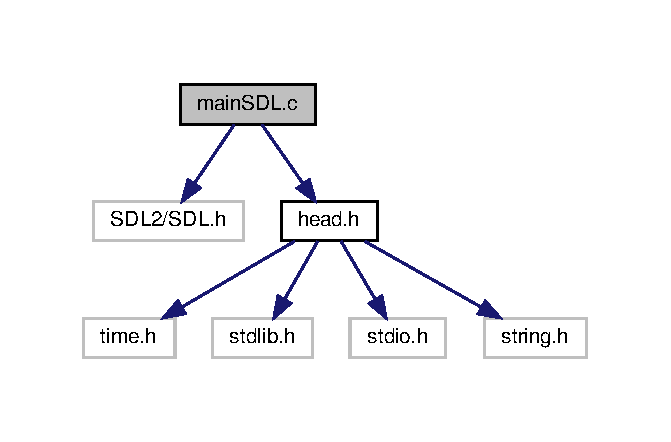
\includegraphics[width=322pt]{mainSDL_8c__incl}
\end{center}
\end{figure}
\subsection*{Data Structures}
\begin{DoxyCompactItemize}
\item 
struct \hyperlink{structcell}{cell}
\begin{DoxyCompactList}\small\item\em gfdjhgf \end{DoxyCompactList}\end{DoxyCompactItemize}
\subsection*{Functions}
\begin{DoxyCompactItemize}
\item 
\hyperlink{structcell}{cell} $\ast$ \hyperlink{mainSDL_8c_a27285143372bf92801396e8ac896e9e2}{init\+Display} (\hyperlink{structcontainer}{container} $\ast$grid, int cell\+Size)
\item 
void \hyperlink{mainSDL_8c_ab961411fd9020c4b2d555cee4b177ab4}{sdl\+Display} (S\+D\+L\+\_\+\+Renderer $\ast$renderer, \hyperlink{structcell}{cell} $\ast$S\+D\+L\+\_\+grid, \hyperlink{structcontainer}{container} $\ast$grid, \hyperlink{structcontainer}{container} $\ast$piece, S\+D\+L\+\_\+\+Color color, int px, int py)
\item 
void \hyperlink{mainSDL_8c_a1e6fb88709bf05a801d646c538927764}{sdl\+Update\+Display} (\hyperlink{structcell}{cell} $\ast$S\+D\+L\+\_\+grid, \hyperlink{structcontainer}{container} $\ast$piece, \hyperlink{structcontainer}{container} $\ast$grid, S\+D\+L\+\_\+\+Color color, int px, int py)
\item 
int \hyperlink{mainSDL_8c_abf9e6b7e6f15df4b525a2e7705ba3089}{main} (int argc, char const $\ast$argv\mbox{[}$\,$\mbox{]})
\end{DoxyCompactItemize}


\subsection{Function Documentation}
\mbox{\Hypertarget{mainSDL_8c_a27285143372bf92801396e8ac896e9e2}\label{mainSDL_8c_a27285143372bf92801396e8ac896e9e2}} 
\index{main\+S\+D\+L.\+c@{main\+S\+D\+L.\+c}!init\+Display@{init\+Display}}
\index{init\+Display@{init\+Display}!main\+S\+D\+L.\+c@{main\+S\+D\+L.\+c}}
\subsubsection{\texorpdfstring{init\+Display()}{initDisplay()}}
{\footnotesize\ttfamily \hyperlink{structcell}{cell} $\ast$ init\+Display (\begin{DoxyParamCaption}\item[{\hyperlink{structcontainer}{container} $\ast$}]{grid,  }\item[{int}]{cell\+Size }\end{DoxyParamCaption})}



Definition at line 110 of file main\+S\+D\+L.\+c.



References cell\+::border, cell\+::cases, container\+::len, and container\+::size.



Referenced by main().


\begin{DoxyCode}
110                                                 \{
111     \hyperlink{structcell}{cell}* SDL\_grid = malloc(\textcolor{keyword}{sizeof}(\hyperlink{structcell}{cell})*grid->\hyperlink{structcontainer_a1e938d250074e70b9778df1b59121744}{size});
112     \textcolor{keywordflow}{for} (\textcolor{keywordtype}{int} y = 0; y < grid->\hyperlink{structcontainer_a1e938d250074e70b9778df1b59121744}{size}/grid->\hyperlink{structcontainer_a0069496fb95c879cd33fb79ab726e81a}{len}; y++) \{
113         \textcolor{keywordflow}{for} (\textcolor{keywordtype}{int} x = 0; x < grid->\hyperlink{structcontainer_a0069496fb95c879cd33fb79ab726e81a}{len}; x++) \{
114             SDL\_grid[(y*grid->\hyperlink{structcontainer_a0069496fb95c879cd33fb79ab726e81a}{len})+x].border.x = 10+((cellSize+2)*x);
115             SDL\_grid[(y*grid->\hyperlink{structcontainer_a0069496fb95c879cd33fb79ab726e81a}{len})+x].border.y = 10+((cellSize+2)*y);
116             SDL\_grid[(y*grid->\hyperlink{structcontainer_a0069496fb95c879cd33fb79ab726e81a}{len})+x].border.h = cellSize+2;
117             SDL\_grid[(y*grid->\hyperlink{structcontainer_a0069496fb95c879cd33fb79ab726e81a}{len})+x].\hyperlink{structcell_ae289d5dfc43a03b47de6dffa417776df}{border}.w = cellSize+2;
118 
119             SDL\_grid[(y*grid->\hyperlink{structcontainer_a0069496fb95c879cd33fb79ab726e81a}{len})+x].cases.x = 10+((cellSize+2)*x)+1;
120             SDL\_grid[(y*grid->\hyperlink{structcontainer_a0069496fb95c879cd33fb79ab726e81a}{len})+x].cases.y = 10+((cellSize+2)*y)+1;
121             SDL\_grid[(y*grid->\hyperlink{structcontainer_a0069496fb95c879cd33fb79ab726e81a}{len})+x].cases.w = cellSize;
122             SDL\_grid[(y*grid->\hyperlink{structcontainer_a0069496fb95c879cd33fb79ab726e81a}{len})+x].\hyperlink{structcell_af2fb9745b37f309905e02fed903748a5}{cases}.h = cellSize;
123 
124             SDL\_grid[(y*grid->\hyperlink{structcontainer_a0069496fb95c879cd33fb79ab726e81a}{len})+x].r = 0;
125             SDL\_grid[(y*grid->\hyperlink{structcontainer_a0069496fb95c879cd33fb79ab726e81a}{len})+x].g = 0;
126             SDL\_grid[(y*grid->\hyperlink{structcontainer_a0069496fb95c879cd33fb79ab726e81a}{len})+x].b = 255;
127         \}
128     \}
129     \textcolor{keywordflow}{return} SDL\_grid;
130 \}
\end{DoxyCode}
Here is the caller graph for this function\+:\nopagebreak
\begin{figure}[H]
\begin{center}
\leavevmode
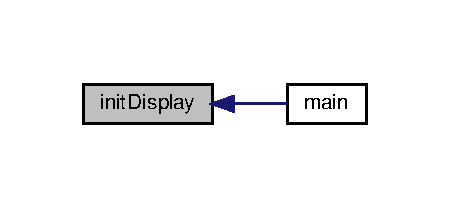
\includegraphics[width=216pt]{mainSDL_8c_a27285143372bf92801396e8ac896e9e2_icgraph}
\end{center}
\end{figure}
\mbox{\Hypertarget{mainSDL_8c_abf9e6b7e6f15df4b525a2e7705ba3089}\label{mainSDL_8c_abf9e6b7e6f15df4b525a2e7705ba3089}} 
\index{main\+S\+D\+L.\+c@{main\+S\+D\+L.\+c}!main@{main}}
\index{main@{main}!main\+S\+D\+L.\+c@{main\+S\+D\+L.\+c}}
\subsubsection{\texorpdfstring{main()}{main()}}
{\footnotesize\ttfamily int main (\begin{DoxyParamCaption}\item[{int}]{argc,  }\item[{char const $\ast$}]{argv\mbox{[}$\,$\mbox{]} }\end{DoxyParamCaption})}



Definition at line 28 of file main\+S\+D\+L.\+c.



References check\+Collision(), H\+E\+I\+G\+HT, init\+Container(), init\+Display(), container\+::len, place(), random\+Piece(), rotate\+\_\+180(), sdl\+Display(), sdl\+Update\+Display(), container\+::size, update(), and W\+I\+D\+TH.


\begin{DoxyCode}
28                                        \{
29 
30     \hyperlink{structcontainer}{container} play\_grid, play\_piece;
31     \textcolor{keywordtype}{int} piece\_x, piece\_y;
32     SDL\_Color color;
33     \hyperlink{structcell}{cell}* SDL\_grid;
34 
35     \textcolor{keywordflow}{if}(SDL\_Init(SDL\_INIT\_VIDEO) != 0) \{
36         printf(\textcolor{stringliteral}{"SDL\_Init error: %s\(\backslash\)n"}, SDL\_GetError());
37         exit(1);
38     \}
39 
40     \hyperlink{container_8c_af20cf8b598b78389dff22b3d176a3727}{initContainer}(\hyperlink{head_8h_a241aeeb764887ae5e3de58b98f04b16d}{WIDTH}, \hyperlink{head_8h_aed89bd71aee8be823e8a20ec4e093c1e}{HEIGHT}, &play\_grid);
41     SDL\_grid = \hyperlink{mainSDL_8c_a27285143372bf92801396e8ac896e9e2}{initDisplay}(&play\_grid,30);
42     \textcolor{keywordflow}{if} (SDL\_grid == NULL) \{
43         printf(\textcolor{stringliteral}{"initDisplay error\(\backslash\)n"});
44         exit(1);
45     \}
46 
47     SDL\_Window* window = NULL;
48     window = SDL\_CreateWindow( \textcolor{stringliteral}{"VapidTetris"}, SDL\_WINDOWPOS\_UNDEFINED, SDL\_WINDOWPOS\_UNDEFINED, 
      \hyperlink{head_8h_a241aeeb764887ae5e3de58b98f04b16d}{WIDTH}*32+20, \hyperlink{head_8h_aed89bd71aee8be823e8a20ec4e093c1e}{HEIGHT}*32+20, SDL\_WINDOW\_SHOWN);
49 
50     SDL\_Renderer* renderer = NULL;
51     renderer =  SDL\_CreateRenderer( window, -1, SDL\_RENDERER\_ACCELERATED);
52 
53     play\_piece = \hyperlink{container_8c_aae1449e449d2f69b52594cccb1dc1e42}{randomPiece}();
54     piece\_x = 0;
55     piece\_y = 0;
56     color.r = 255;
57     color.g = 0;
58     color.b = 0;
59 
60     \hyperlink{mainSDL_8c_ab961411fd9020c4b2d555cee4b177ab4}{sdlDisplay}(renderer, SDL\_grid, &play\_grid, &play\_piece, color, piece\_x, piece\_y);
61 
62     \textcolor{keywordtype}{int} tmp = 1;
63     \textcolor{keywordflow}{while} (tmp) \{
64         SDL\_Event event;
65         SDL\_PollEvent(&event);
66         \textcolor{keywordflow}{switch} (event.type) \{
67             \textcolor{keywordflow}{case} SDL\_KEYDOWN:
68                 \textcolor{keywordflow}{switch}(event.key.keysym.sym) \{
69                     \textcolor{keywordflow}{case} \textcolor{charliteral}{'q'}: piece\_x-=1; \textcolor{keywordflow}{break};
70                     \textcolor{keywordflow}{case} \textcolor{charliteral}{'d'}: piece\_x+=1; \textcolor{keywordflow}{break};
71                     \textcolor{keywordflow}{case} \textcolor{charliteral}{'z'}: piece\_y-=1; \textcolor{keywordflow}{break};
72                     \textcolor{keywordflow}{case} \textcolor{charliteral}{'s'}: piece\_y+=1; \textcolor{keywordflow}{break};
73                     \textcolor{keywordflow}{case} \textcolor{charliteral}{'r'}: \hyperlink{head_8h_afbdf40ca68538464d0df29d9b2a77366}{rotate\_180}(&play\_piece); \textcolor{keywordflow}{break};
74                     \textcolor{keywordflow}{case} \textcolor{charliteral}{'p'}:
75                         \textcolor{keywordflow}{if} (\hyperlink{container_8c_a7a74c6812adffb8d4419092b999a823b}{checkCollision}(&play\_grid, &play\_piece, piece\_x, piece\_y)) \{
76                             printf(\textcolor{stringliteral}{"Can't fit here!\(\backslash\)n"});
77                         \}\textcolor{keywordflow}{else}\{
78                             \hyperlink{container_8c_a46bfac7d0493d39bd4aad51f270bd0d7}{place}(&play\_grid, &play\_piece, piece\_x, piece\_y);
79                             \hyperlink{mainSDL_8c_a1e6fb88709bf05a801d646c538927764}{sdlUpdateDisplay}(SDL\_grid,&play\_piece,&play\_grid, color, 
      piece\_x, piece\_y);
80                             play\_piece = \hyperlink{container_8c_aae1449e449d2f69b52594cccb1dc1e42}{randomPiece}();
81                             \hyperlink{head_8h_aca3f584034ddadfcf89951a1bf10f45c}{update}(&play\_grid);
82                         \}
83                         \textcolor{keywordflow}{break};
84                 \}
85                 \textcolor{keywordflow}{if} (piece\_x<0) \{
86                     piece\_x = 0;
87                 \}
88                 \textcolor{keywordflow}{if} (piece\_y<0) \{
89                     piece\_y = 0;
90                 \}
91                 \textcolor{keywordflow}{if} (piece\_x>play\_grid.\hyperlink{structcontainer_a0069496fb95c879cd33fb79ab726e81a}{len}-play\_piece.\hyperlink{structcontainer_a0069496fb95c879cd33fb79ab726e81a}{len}) \{
92                     piece\_x = play\_grid.\hyperlink{structcontainer_a0069496fb95c879cd33fb79ab726e81a}{len}-play\_piece.\hyperlink{structcontainer_a0069496fb95c879cd33fb79ab726e81a}{len};
93                 \}
94                 \textcolor{keywordflow}{if} (piece\_y>(play\_grid.\hyperlink{structcontainer_a1e938d250074e70b9778df1b59121744}{size}/play\_grid.\hyperlink{structcontainer_a0069496fb95c879cd33fb79ab726e81a}{len})-(play\_piece.
      \hyperlink{structcontainer_a1e938d250074e70b9778df1b59121744}{size}/play\_piece.\hyperlink{structcontainer_a0069496fb95c879cd33fb79ab726e81a}{len})) \{
95                     piece\_y = (play\_grid.\hyperlink{structcontainer_a1e938d250074e70b9778df1b59121744}{size}/play\_grid.\hyperlink{structcontainer_a0069496fb95c879cd33fb79ab726e81a}{len})-(play\_piece.
      \hyperlink{structcontainer_a1e938d250074e70b9778df1b59121744}{size}/play\_piece.\hyperlink{structcontainer_a0069496fb95c879cd33fb79ab726e81a}{len});
96                 \}
97                 \hyperlink{mainSDL_8c_ab961411fd9020c4b2d555cee4b177ab4}{sdlDisplay}(renderer, SDL\_grid, &play\_grid, &play\_piece, color, piece\_x, piece\_y);
98                 \textcolor{keywordflow}{break};
99             \textcolor{keywordflow}{case} SDL\_QUIT:
100                 tmp = 0;
101                 \textcolor{keywordflow}{break};
102             default :
103                 \textcolor{keywordflow}{break};
104         \}
105     \}
106 
107     \textcolor{keywordflow}{return} 0;
108 \}
\end{DoxyCode}
Here is the call graph for this function\+:\nopagebreak
\begin{figure}[H]
\begin{center}
\leavevmode
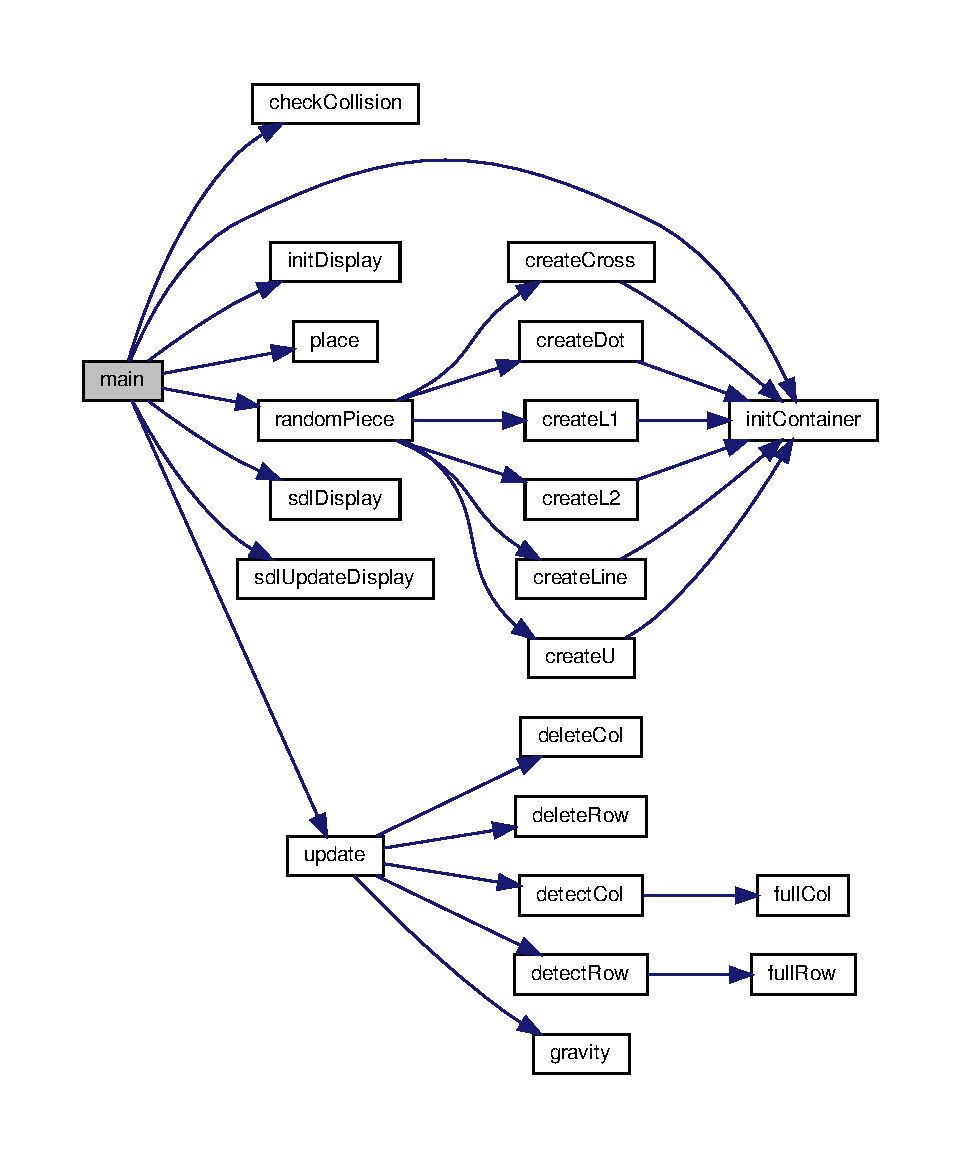
\includegraphics[width=350pt]{mainSDL_8c_abf9e6b7e6f15df4b525a2e7705ba3089_cgraph}
\end{center}
\end{figure}
\mbox{\Hypertarget{mainSDL_8c_ab961411fd9020c4b2d555cee4b177ab4}\label{mainSDL_8c_ab961411fd9020c4b2d555cee4b177ab4}} 
\index{main\+S\+D\+L.\+c@{main\+S\+D\+L.\+c}!sdl\+Display@{sdl\+Display}}
\index{sdl\+Display@{sdl\+Display}!main\+S\+D\+L.\+c@{main\+S\+D\+L.\+c}}
\subsubsection{\texorpdfstring{sdl\+Display()}{sdlDisplay()}}
{\footnotesize\ttfamily void sdl\+Display (\begin{DoxyParamCaption}\item[{S\+D\+L\+\_\+\+Renderer $\ast$}]{renderer,  }\item[{\hyperlink{structcell}{cell} $\ast$}]{S\+D\+L\+\_\+grid,  }\item[{\hyperlink{structcontainer}{container} $\ast$}]{grid,  }\item[{\hyperlink{structcontainer}{container} $\ast$}]{piece,  }\item[{S\+D\+L\+\_\+\+Color}]{color,  }\item[{int}]{px,  }\item[{int}]{py }\end{DoxyParamCaption})}



Definition at line 145 of file main\+S\+D\+L.\+c.



References cell\+::border, cell\+::cases, container\+::data, container\+::len, and container\+::size.



Referenced by main().


\begin{DoxyCode}
145                                                                                                            
                       \{
146 
147     \textcolor{keywordflow}{for} (\textcolor{keywordtype}{int} y = 0; y < (grid->\hyperlink{structcontainer_a1e938d250074e70b9778df1b59121744}{size}/grid->\hyperlink{structcontainer_a0069496fb95c879cd33fb79ab726e81a}{len}); y++) \{
148         \textcolor{keywordflow}{for} (\textcolor{keywordtype}{int} x = 0; x < grid->\hyperlink{structcontainer_a0069496fb95c879cd33fb79ab726e81a}{len}; x++) \{
149 
150             \textcolor{keywordflow}{if} (x>=px && x<(px+piece->\hyperlink{structcontainer_a0069496fb95c879cd33fb79ab726e81a}{len}) && y>=py && y<(py+(piece->\hyperlink{structcontainer_a1e938d250074e70b9778df1b59121744}{size}/piece->
      \hyperlink{structcontainer_a0069496fb95c879cd33fb79ab726e81a}{len})) && piece->\hyperlink{structcontainer_aefae69762fe9c24169e2ca5418a711a1}{data}[((y-py)*piece->\hyperlink{structcontainer_a0069496fb95c879cd33fb79ab726e81a}{len})+x-px]) \{
151                 SDL\_SetRenderDrawColor( renderer, color.r, color.g, color.b, 255 );
152             \}\textcolor{keywordflow}{else}\{
153                 SDL\_SetRenderDrawColor( renderer, 0, 0, 0, 255 );
154             \}
155             SDL\_RenderFillRect( renderer, &(SDL\_grid[(y*grid->\hyperlink{structcontainer_a0069496fb95c879cd33fb79ab726e81a}{len})+x].\hyperlink{structcell_ae289d5dfc43a03b47de6dffa417776df}{border}));
156 
157             \textcolor{keywordflow}{if}(grid->\hyperlink{structcontainer_aefae69762fe9c24169e2ca5418a711a1}{data}[(y*grid->\hyperlink{structcontainer_a0069496fb95c879cd33fb79ab726e81a}{len})+x] == 1)\{
158                 SDL\_SetRenderDrawColor( renderer, 255, 0, 0, 255 );
159             \}
160             \textcolor{keywordflow}{else} \textcolor{keywordflow}{if}(grid->\hyperlink{structcontainer_aefae69762fe9c24169e2ca5418a711a1}{data}[(y*grid->\hyperlink{structcontainer_a0069496fb95c879cd33fb79ab726e81a}{len})+x] == 2)\{
161                 SDL\_SetRenderDrawColor( renderer, 0, 255, 0, 255 );
162             \}
163             \textcolor{keywordflow}{else} \textcolor{keywordflow}{if}(grid->\hyperlink{structcontainer_aefae69762fe9c24169e2ca5418a711a1}{data}[(y*grid->\hyperlink{structcontainer_a0069496fb95c879cd33fb79ab726e81a}{len})+x] == 3)\{
164                 SDL\_SetRenderDrawColor( renderer, 0, 0, 255, 255 );
165             \}
166             \textcolor{keywordflow}{else} \textcolor{keywordflow}{if}(grid->\hyperlink{structcontainer_aefae69762fe9c24169e2ca5418a711a1}{data}[(y*grid->\hyperlink{structcontainer_a0069496fb95c879cd33fb79ab726e81a}{len})+x] == 4)\{
167                 SDL\_SetRenderDrawColor( renderer, 255, 255, 0, 255 );
168             \}
169             \textcolor{keywordflow}{else} \textcolor{keywordflow}{if}(grid->\hyperlink{structcontainer_aefae69762fe9c24169e2ca5418a711a1}{data}[(y*grid->\hyperlink{structcontainer_a0069496fb95c879cd33fb79ab726e81a}{len})+x] == 5)\{
170                 SDL\_SetRenderDrawColor( renderer, 255, 0, 255, 255 );
171             \}
172             \textcolor{keywordflow}{else} \textcolor{keywordflow}{if}(grid->\hyperlink{structcontainer_aefae69762fe9c24169e2ca5418a711a1}{data}[(y*grid->\hyperlink{structcontainer_a0069496fb95c879cd33fb79ab726e81a}{len})+x] == 6)\{
173                 SDL\_SetRenderDrawColor( renderer, 0, 255, 255, 255 );
174             \}
175             \textcolor{keywordflow}{else}\{
176                 SDL\_SetRenderDrawColor( renderer, 123, 123, 123, 255 );
177             \}
178                 SDL\_RenderFillRect( renderer, &(SDL\_grid[(y*grid->\hyperlink{structcontainer_a0069496fb95c879cd33fb79ab726e81a}{len})+x].
      \hyperlink{structcell_af2fb9745b37f309905e02fed903748a5}{cases}));
179         \}
180     \}
181     SDL\_RenderPresent(renderer);
182 \}
\end{DoxyCode}
Here is the caller graph for this function\+:\nopagebreak
\begin{figure}[H]
\begin{center}
\leavevmode
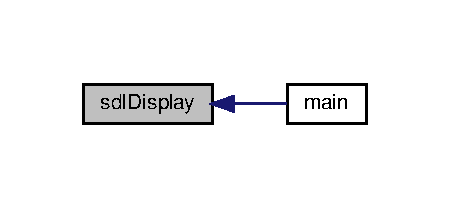
\includegraphics[width=216pt]{mainSDL_8c_ab961411fd9020c4b2d555cee4b177ab4_icgraph}
\end{center}
\end{figure}
\mbox{\Hypertarget{mainSDL_8c_a1e6fb88709bf05a801d646c538927764}\label{mainSDL_8c_a1e6fb88709bf05a801d646c538927764}} 
\index{main\+S\+D\+L.\+c@{main\+S\+D\+L.\+c}!sdl\+Update\+Display@{sdl\+Update\+Display}}
\index{sdl\+Update\+Display@{sdl\+Update\+Display}!main\+S\+D\+L.\+c@{main\+S\+D\+L.\+c}}
\subsubsection{\texorpdfstring{sdl\+Update\+Display()}{sdlUpdateDisplay()}}
{\footnotesize\ttfamily void sdl\+Update\+Display (\begin{DoxyParamCaption}\item[{\hyperlink{structcell}{cell} $\ast$}]{S\+D\+L\+\_\+grid,  }\item[{\hyperlink{structcontainer}{container} $\ast$}]{piece,  }\item[{\hyperlink{structcontainer}{container} $\ast$}]{grid,  }\item[{S\+D\+L\+\_\+\+Color}]{color,  }\item[{int}]{px,  }\item[{int}]{py }\end{DoxyParamCaption})}



Definition at line 132 of file main\+S\+D\+L.\+c.



References container\+::data, container\+::len, and container\+::size.



Referenced by main().


\begin{DoxyCode}
132                                                                                                         \{
133     \textcolor{keywordtype}{int} y, x;
134     \textcolor{keywordflow}{for} (y = 0; y < grid->\hyperlink{structcontainer_a1e938d250074e70b9778df1b59121744}{size}/grid->\hyperlink{structcontainer_a0069496fb95c879cd33fb79ab726e81a}{len}; y++) \{
135         \textcolor{keywordflow}{for} (x = 0; x < grid->\hyperlink{structcontainer_a0069496fb95c879cd33fb79ab726e81a}{len}; x++) \{
136             \textcolor{keywordflow}{if} (x>=px && x<(px+piece->\hyperlink{structcontainer_a0069496fb95c879cd33fb79ab726e81a}{len}) && y>=py && y<(py+(piece->\hyperlink{structcontainer_a1e938d250074e70b9778df1b59121744}{size}/piece->
      \hyperlink{structcontainer_a0069496fb95c879cd33fb79ab726e81a}{len})) && piece->\hyperlink{structcontainer_aefae69762fe9c24169e2ca5418a711a1}{data}[((y-py)*piece->\hyperlink{structcontainer_a0069496fb95c879cd33fb79ab726e81a}{len})+x-px]) \{
137                 SDL\_grid[(y*grid->\hyperlink{structcontainer_a0069496fb95c879cd33fb79ab726e81a}{len})+x].r = color.r;
138                 SDL\_grid[(y*grid->\hyperlink{structcontainer_a0069496fb95c879cd33fb79ab726e81a}{len})+x].g = color.g;
139                 SDL\_grid[(y*grid->\hyperlink{structcontainer_a0069496fb95c879cd33fb79ab726e81a}{len})+x].b = color.b;
140             \}
141         \}
142     \}
143 \}
\end{DoxyCode}
Here is the caller graph for this function\+:\nopagebreak
\begin{figure}[H]
\begin{center}
\leavevmode
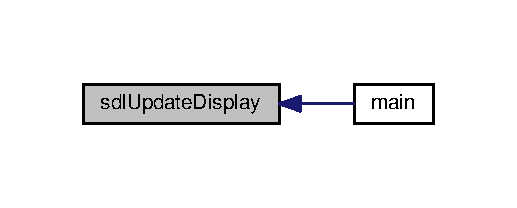
\includegraphics[width=248pt]{mainSDL_8c_a1e6fb88709bf05a801d646c538927764_icgraph}
\end{center}
\end{figure}

\hypertarget{README_8md}{}\section{R\+E\+A\+D\+M\+E.\+md File Reference}
\label{README_8md}\index{R\+E\+A\+D\+M\+E.\+md@{R\+E\+A\+D\+M\+E.\+md}}

\hypertarget{update_8c}{}\section{update.\+c File Reference}
\label{update_8c}\index{update.\+c@{update.\+c}}
{\ttfamily \#include \char`\"{}head.\+h\char`\"{}}\newline
Include dependency graph for update.\+c\+:
% FIG 0
\subsection*{Functions}
\begin{DoxyCompactItemize}
\item 
int $\ast$ \hyperlink{update_8c_af9526652ed9443df3955c6cac0fe12c7}{detect\+Row} (\hyperlink{structcontainer}{container} $\ast$grid)
\item 
char \hyperlink{update_8c_a35c79938c8ccc4683d509620aa6e15af}{full\+Row} (\hyperlink{structcontainer}{container} $\ast$grid, int index)
\item 
void \hyperlink{update_8c_ab48ae1a72cd2b7ff673d732f26d74ce0}{delete\+Row} (\hyperlink{structcontainer}{container} $\ast$grid, int $\ast$index\+\_\+list)
\item 
int $\ast$ \hyperlink{update_8c_a0e35a2936fc69af30890ce30a082b594}{detect\+Col} (\hyperlink{structcontainer}{container} $\ast$grid)
\item 
char \hyperlink{update_8c_aebb74ac9ba3f8c734beba4617a6bf439}{full\+Col} (\hyperlink{structcontainer}{container} $\ast$grid, int index)
\item 
void \hyperlink{update_8c_aa4713ce5d04fcf86179bc68fbd9bdbd4}{delete\+Col} (\hyperlink{structcontainer}{container} $\ast$grid, int $\ast$index\+\_\+list)
\item 
void \hyperlink{update_8c_a4fa6bbed60f00a099cdd9d5d047c8a46}{gravity} (\hyperlink{structcontainer}{container} $\ast$grid, int $\ast$index\+\_\+list\+\_\+row, int $\ast$index\+\_\+list\+\_\+col)
\item 
void \hyperlink{update_8c_aca3f584034ddadfcf89951a1bf10f45c}{update} (\hyperlink{structcontainer}{container} $\ast$grid)
\end{DoxyCompactItemize}


\subsection{Function Documentation}
\mbox{\Hypertarget{update_8c_aa4713ce5d04fcf86179bc68fbd9bdbd4}\label{update_8c_aa4713ce5d04fcf86179bc68fbd9bdbd4}} 
\index{update.\+c@{update.\+c}!delete\+Col@{delete\+Col}}
\index{delete\+Col@{delete\+Col}!update.\+c@{update.\+c}}
\subsubsection{\texorpdfstring{delete\+Col()}{deleteCol()}}
{\footnotesize\ttfamily void delete\+Col (\begin{DoxyParamCaption}\item[{\hyperlink{structcontainer}{container} $\ast$}]{grid,  }\item[{int $\ast$}]{index\+\_\+list }\end{DoxyParamCaption})}



Definition at line 108 of file update.\+c.



References container\+::data, container\+::len, and container\+::size.



Referenced by update().


\begin{DoxyCode}
108                                                 \{
109 
110     \textcolor{keywordtype}{int} actual, max\_len, max\_size, max\_size1, i, j;
111     \textcolor{keywordtype}{char} *save\_data;
112 
113     \textcolor{comment}{//Sauvegarde}
114     save\_data = grid->\hyperlink{structcontainer_aefae69762fe9c24169e2ca5418a711a1}{data};
115     max\_len = grid->\hyperlink{structcontainer_a0069496fb95c879cd33fb79ab726e81a}{len};
116     max\_size1 = grid->\hyperlink{structcontainer_a1e938d250074e70b9778df1b59121744}{size};
117 
118     max\_size = index\_list[0];
119 
120     \textcolor{keywordflow}{for}(i=1; i<max\_size; ++i)\{
121         actual = index\_list[i];
122         \textcolor{keywordflow}{for}(j=actual; j< max\_size1; j += max\_len)\{
123             save\_data[j] = 0;
124         \}
125     \}
126 
127 \}
\end{DoxyCode}
Here is the caller graph for this function\+:
% FIG 1
\mbox{\Hypertarget{update_8c_ab48ae1a72cd2b7ff673d732f26d74ce0}\label{update_8c_ab48ae1a72cd2b7ff673d732f26d74ce0}} 
\index{update.\+c@{update.\+c}!delete\+Row@{delete\+Row}}
\index{delete\+Row@{delete\+Row}!update.\+c@{update.\+c}}
\subsubsection{\texorpdfstring{delete\+Row()}{deleteRow()}}
{\footnotesize\ttfamily void delete\+Row (\begin{DoxyParamCaption}\item[{\hyperlink{structcontainer}{container} $\ast$}]{grid,  }\item[{int $\ast$}]{index\+\_\+list }\end{DoxyParamCaption})}



Definition at line 44 of file update.\+c.



References container\+::data, and container\+::len.



Referenced by update().


\begin{DoxyCode}
44                                                 \{
45 
46     \textcolor{keywordtype}{int} actual, max\_len, max\_size, i, j;
47     \textcolor{keywordtype}{char} *save\_data;
48 
49     \textcolor{comment}{//Sauvegarde}
50     save\_data = grid->\hyperlink{structcontainer_aefae69762fe9c24169e2ca5418a711a1}{data};
51     max\_len = grid->\hyperlink{structcontainer_a0069496fb95c879cd33fb79ab726e81a}{len};
52 
53     max\_size = index\_list[0];
54     \textcolor{keywordflow}{for}(i=1; i<max\_size; ++i)\{
55         actual = index\_list[i];
56         \textcolor{keywordflow}{for}(j=actual; j< actual + max\_len; ++j)\{
57             save\_data[j] = 0;
58         \}
59     \}
60 
61 \}
\end{DoxyCode}
Here is the caller graph for this function\+:
% FIG 2
\mbox{\Hypertarget{update_8c_a0e35a2936fc69af30890ce30a082b594}\label{update_8c_a0e35a2936fc69af30890ce30a082b594}} 
\index{update.\+c@{update.\+c}!detect\+Col@{detect\+Col}}
\index{detect\+Col@{detect\+Col}!update.\+c@{update.\+c}}
\subsubsection{\texorpdfstring{detect\+Col()}{detectCol()}}
{\footnotesize\ttfamily int$\ast$ detect\+Col (\begin{DoxyParamCaption}\item[{\hyperlink{structcontainer}{container} $\ast$}]{grid }\end{DoxyParamCaption})}



Definition at line 66 of file update.\+c.



References full\+Col(), and container\+::len.



Referenced by update().


\begin{DoxyCode}
66                                \{
67 
68     \textcolor{keywordtype}{int} *index, actual, max\_len, i;
69 
70     \textcolor{comment}{//save}
71     max\_len = grid->\hyperlink{structcontainer_a0069496fb95c879cd33fb79ab726e81a}{len};
72 
73     \textcolor{comment}{//Index}
74     actual = 1;
75     index = malloc((max\_len+1)*\textcolor{keyword}{sizeof}(\textcolor{keywordtype}{int}));
76 
77     \textcolor{keywordflow}{for}(i=0; i<max\_len; ++i)\{
78         \textcolor{keywordflow}{if}(\hyperlink{update_8c_aebb74ac9ba3f8c734beba4617a6bf439}{fullCol}(grid, i))\{
79             index[actual] = i;
80             ++actual;
81         \}
82     \}
83 
84     index[0] = actual;
85 
86     \textcolor{keywordflow}{return} realloc(index, actual);
87 \}
\end{DoxyCode}
Here is the call graph for this function\+:
% FIG 3
Here is the caller graph for this function\+:
% FIG 4
\mbox{\Hypertarget{update_8c_af9526652ed9443df3955c6cac0fe12c7}\label{update_8c_af9526652ed9443df3955c6cac0fe12c7}} 
\index{update.\+c@{update.\+c}!detect\+Row@{detect\+Row}}
\index{detect\+Row@{detect\+Row}!update.\+c@{update.\+c}}
\subsubsection{\texorpdfstring{detect\+Row()}{detectRow()}}
{\footnotesize\ttfamily int$\ast$ detect\+Row (\begin{DoxyParamCaption}\item[{\hyperlink{structcontainer}{container} $\ast$}]{grid }\end{DoxyParamCaption})}



Definition at line 4 of file update.\+c.



References full\+Row(), container\+::len, and container\+::size.



Referenced by update().


\begin{DoxyCode}
4                                \{
5 
6     \textcolor{keywordtype}{int} *index, actual, max\_len, max\_size, i;
7 
8     \textcolor{comment}{//Sauvegarde}
9     max\_len = grid->\hyperlink{structcontainer_a0069496fb95c879cd33fb79ab726e81a}{len};
10     max\_size = grid->\hyperlink{structcontainer_a1e938d250074e70b9778df1b59121744}{size};
11 
12     \textcolor{comment}{//Index}
13     actual = 1;
14     index = malloc((max\_size/max\_len + 1)*\textcolor{keyword}{sizeof}(\textcolor{keywordtype}{int}));
15 
16     \textcolor{keywordflow}{for}(i=0; i<max\_size; i += max\_len)\{
17         \textcolor{keywordflow}{if}(\hyperlink{update_8c_a35c79938c8ccc4683d509620aa6e15af}{fullRow}(grid, i))\{
18             index[actual] = i;
19             ++actual;
20         \}
21     \}
22     index[0] = actual;
23 
24     \textcolor{keywordflow}{return} realloc(index, actual);
25 \}
\end{DoxyCode}
Here is the call graph for this function\+:
% FIG 5
Here is the caller graph for this function\+:
% FIG 6
\mbox{\Hypertarget{update_8c_aebb74ac9ba3f8c734beba4617a6bf439}\label{update_8c_aebb74ac9ba3f8c734beba4617a6bf439}} 
\index{update.\+c@{update.\+c}!full\+Col@{full\+Col}}
\index{full\+Col@{full\+Col}!update.\+c@{update.\+c}}
\subsubsection{\texorpdfstring{full\+Col()}{fullCol()}}
{\footnotesize\ttfamily char full\+Col (\begin{DoxyParamCaption}\item[{\hyperlink{structcontainer}{container} $\ast$}]{grid,  }\item[{int}]{index }\end{DoxyParamCaption})}



Definition at line 89 of file update.\+c.



References container\+::data, container\+::len, and container\+::size.



Referenced by detect\+Col().


\begin{DoxyCode}
89                                         \{
90 
91     \textcolor{keywordtype}{int} max\_size, max\_len, j;
92     \textcolor{keywordtype}{char}* save\_data;
93 
94     \textcolor{comment}{//save}
95     save\_data = grid->\hyperlink{structcontainer_aefae69762fe9c24169e2ca5418a711a1}{data};
96     max\_size = grid->\hyperlink{structcontainer_a1e938d250074e70b9778df1b59121744}{size};
97     max\_len = grid->\hyperlink{structcontainer_a0069496fb95c879cd33fb79ab726e81a}{len};
98 
99     \textcolor{keywordflow}{for}(j=index; j<max\_size; j+=max\_len)\{
100         \textcolor{keywordflow}{if}(save\_data[j] != 1) \textcolor{keywordflow}{break};
101     \}
102     \textcolor{keywordflow}{if}(j >= max\_size)\{
103         \textcolor{keywordflow}{return} 1;
104     \}
105     \textcolor{keywordflow}{return} 0;
106 \}
\end{DoxyCode}
Here is the caller graph for this function\+:
% FIG 7
\mbox{\Hypertarget{update_8c_a35c79938c8ccc4683d509620aa6e15af}\label{update_8c_a35c79938c8ccc4683d509620aa6e15af}} 
\index{update.\+c@{update.\+c}!full\+Row@{full\+Row}}
\index{full\+Row@{full\+Row}!update.\+c@{update.\+c}}
\subsubsection{\texorpdfstring{full\+Row()}{fullRow()}}
{\footnotesize\ttfamily char full\+Row (\begin{DoxyParamCaption}\item[{\hyperlink{structcontainer}{container} $\ast$}]{grid,  }\item[{int}]{index }\end{DoxyParamCaption})}



Definition at line 27 of file update.\+c.



References container\+::data, and container\+::len.



Referenced by detect\+Row().


\begin{DoxyCode}
27                                         \{
28 
29     \textcolor{keywordtype}{int} max\_len, j;
30     \textcolor{keywordtype}{char}* save\_data;
31 
32     save\_data = grid->\hyperlink{structcontainer_aefae69762fe9c24169e2ca5418a711a1}{data};
33     max\_len = grid->\hyperlink{structcontainer_a0069496fb95c879cd33fb79ab726e81a}{len};
34 
35     \textcolor{keywordflow}{for}(j=index; j< index + max\_len; ++j)\{
36         \textcolor{keywordflow}{if}(save\_data[j] != 1) \textcolor{keywordflow}{break};
37     \}
38     \textcolor{keywordflow}{if}(j == index + max\_len)\{
39         \textcolor{keywordflow}{return} 1;
40     \}
41     \textcolor{keywordflow}{return} 0;
42 \}
\end{DoxyCode}
Here is the caller graph for this function\+:
% FIG 8
\mbox{\Hypertarget{update_8c_a4fa6bbed60f00a099cdd9d5d047c8a46}\label{update_8c_a4fa6bbed60f00a099cdd9d5d047c8a46}} 
\index{update.\+c@{update.\+c}!gravity@{gravity}}
\index{gravity@{gravity}!update.\+c@{update.\+c}}
\subsubsection{\texorpdfstring{gravity()}{gravity()}}
{\footnotesize\ttfamily void gravity (\begin{DoxyParamCaption}\item[{\hyperlink{structcontainer}{container} $\ast$}]{grid,  }\item[{int $\ast$}]{index\+\_\+list\+\_\+row,  }\item[{int $\ast$}]{index\+\_\+list\+\_\+col }\end{DoxyParamCaption})}



Definition at line 130 of file update.\+c.



References container\+::data, container\+::len, and container\+::size.



Referenced by update().


\begin{DoxyCode}
130                                                                        \{
131 
132     \textcolor{keywordtype}{int} max\_len, max\_size, save\_size, save\_index, i, j, k;
133     \textcolor{keywordtype}{char} *save\_data;
134 
135     \textcolor{comment}{//Save}
136     save\_data = grid->\hyperlink{structcontainer_aefae69762fe9c24169e2ca5418a711a1}{data};
137     max\_size = grid->\hyperlink{structcontainer_a1e938d250074e70b9778df1b59121744}{size};
138     max\_len = grid->\hyperlink{structcontainer_a0069496fb95c879cd33fb79ab726e81a}{len};
139 
140     \textcolor{comment}{//Update row}
141     save\_size = index\_list\_row[0];
142     \textcolor{keywordflow}{for}(i=1; i<save\_size; ++i)\{
143         \textcolor{keywordflow}{for}(j=index\_list\_row[i]-1; j>=0; --j)\{
144             save\_data[j+max\_len] = save\_data[j];
145             save\_data[j] = 0;
146         \}
147     \}
148 
149     \textcolor{comment}{//Update Col}
150     save\_size = index\_list\_col[0];
151     \textcolor{keywordflow}{for}(i=save\_size-1; i>=1; --i)\{
152         save\_index = index\_list\_col[i];
153         \textcolor{keywordflow}{for}(j=0; j<max\_size; j += max\_len)\{
154             \textcolor{keywordflow}{for}(k=save\_index + j + 1; k < max\_len + j; ++k)\{
155                 save\_data[k-1] = save\_data[k];
156                 save\_data[k] = 0;
157             \}
158         \}
159     \}
160 
161 \}
\end{DoxyCode}
Here is the caller graph for this function\+:
% FIG 9
\mbox{\Hypertarget{update_8c_aca3f584034ddadfcf89951a1bf10f45c}\label{update_8c_aca3f584034ddadfcf89951a1bf10f45c}} 
\index{update.\+c@{update.\+c}!update@{update}}
\index{update@{update}!update.\+c@{update.\+c}}
\subsubsection{\texorpdfstring{update()}{update()}}
{\footnotesize\ttfamily void update (\begin{DoxyParamCaption}\item[{\hyperlink{structcontainer}{container} $\ast$}]{grid }\end{DoxyParamCaption})}



Definition at line 164 of file update.\+c.



References delete\+Col(), delete\+Row(), detect\+Col(), detect\+Row(), and gravity().



Referenced by main().


\begin{DoxyCode}
164                             \{
165     \textcolor{keywordtype}{int} *index\_list\_row, *index\_list\_col;
166     index\_list\_row = \hyperlink{update_8c_af9526652ed9443df3955c6cac0fe12c7}{detectRow}(grid);
167     index\_list\_col = \hyperlink{update_8c_a0e35a2936fc69af30890ce30a082b594}{detectCol}(grid);
168 
169     \hyperlink{update_8c_ab48ae1a72cd2b7ff673d732f26d74ce0}{deleteRow}(grid, index\_list\_row);
170     \hyperlink{update_8c_aa4713ce5d04fcf86179bc68fbd9bdbd4}{deleteCol}(grid, index\_list\_col);
171 
172     \hyperlink{update_8c_a4fa6bbed60f00a099cdd9d5d047c8a46}{gravity}(grid, index\_list\_row, index\_list\_col);
173 
174     free(index\_list\_row);
175     free(index\_list\_col);
176 \}
\end{DoxyCode}
Here is the call graph for this function\+:
% FIG 10
Here is the caller graph for this function\+:
% FIG 11

\hypertarget{user_8c}{}\section{user.\+c File Reference}
\label{user_8c}\index{user.\+c@{user.\+c}}
{\ttfamily \#include \char`\"{}head.\+h\char`\"{}}\newline
Include dependency graph for user.\+c\+:
\nopagebreak
\begin{figure}[H]
\begin{center}
\leavevmode
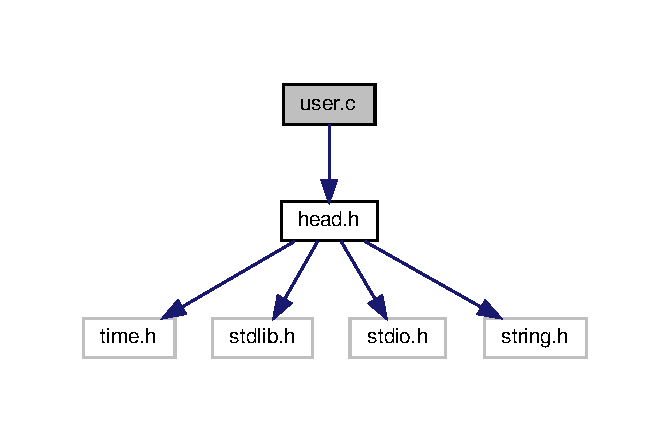
\includegraphics[width=322pt]{user_8c__incl}
\end{center}
\end{figure}
\subsection*{Functions}
\begin{DoxyCompactItemize}
\item 
void \hyperlink{user_8c_ac2b3cb6c7ec0748f0c4c1a46e0997d70}{display} (\hyperlink{structcontainer}{container} $\ast$grid)
\item 
void \hyperlink{user_8c_afbdf40ca68538464d0df29d9b2a77366}{rotate\+\_\+180} (\hyperlink{structcontainer}{container} $\ast$piece)
\item 
void \hyperlink{user_8c_a44fa0cbfa7fc79473c8ac9ca3b198f5a}{rotate\+\_\+90} (\hyperlink{structcontainer}{container} $\ast$piece)
\end{DoxyCompactItemize}


\subsection{Function Documentation}
\mbox{\Hypertarget{user_8c_ac2b3cb6c7ec0748f0c4c1a46e0997d70}\label{user_8c_ac2b3cb6c7ec0748f0c4c1a46e0997d70}} 
\index{user.\+c@{user.\+c}!display@{display}}
\index{display@{display}!user.\+c@{user.\+c}}
\subsubsection{\texorpdfstring{display()}{display()}}
{\footnotesize\ttfamily void display (\begin{DoxyParamCaption}\item[{\hyperlink{structcontainer}{container} $\ast$}]{grid }\end{DoxyParamCaption})}



Definition at line 3 of file user.\+c.



References container\+::data, container\+::len, and container\+::size.



Referenced by main().


\begin{DoxyCode}
3                              \{
4     \textcolor{keywordtype}{char} *toShow = \textcolor{stringliteral}{"36m"};
5     \textcolor{keywordtype}{int} i;
6 
7     \textcolor{keywordflow}{for} (i = 0; i < grid->\hyperlink{structcontainer_a0069496fb95c879cd33fb79ab726e81a}{len}+2; i++) \{
8         printf(\textcolor{stringliteral}{"-"});
9     \}
10     printf(\textcolor{stringliteral}{"\(\backslash\)n|"});
11 
12     \textcolor{keywordflow}{for} (i = 0; i < grid->\hyperlink{structcontainer_a1e938d250074e70b9778df1b59121744}{size}; i++) \{
13         \textcolor{keywordflow}{if} (i % grid->\hyperlink{structcontainer_a0069496fb95c879cd33fb79ab726e81a}{len} == 0 && i != 0) \{
14             printf(\textcolor{stringliteral}{"|%d\(\backslash\)n|"}, (i/grid->\hyperlink{structcontainer_a0069496fb95c879cd33fb79ab726e81a}{len})-1);  \textcolor{comment}{// Erreur ! Affichage de 23 puis 25 dans les deux
       dernières lignes de la zone de jeu, et même phénomène pour la preview pièce}
15         \}
16 
17         \textcolor{keywordflow}{switch} (grid->\hyperlink{structcontainer_aefae69762fe9c24169e2ca5418a711a1}{data}[i]) \{
18             \textcolor{keywordflow}{case} 2:
19                 toShow = \textcolor{stringliteral}{"31m"};
20                 \textcolor{keywordflow}{break};
21         \}
22 
23         \textcolor{keywordflow}{if} (grid->\hyperlink{structcontainer_aefae69762fe9c24169e2ca5418a711a1}{data}[i] > 0)\{
24             printf(\textcolor{stringliteral}{"\(\backslash\)033[%sX"}, toShow);
25         \}\textcolor{keywordflow}{else}\{
26             printf(\textcolor{stringliteral}{" "});
27         \}
28     \}
29     printf(\textcolor{stringliteral}{"|%d\(\backslash\)n"},i/grid->\hyperlink{structcontainer_a0069496fb95c879cd33fb79ab726e81a}{len}-1);
30     \textcolor{keywordflow}{for} (i = 0; i < grid->\hyperlink{structcontainer_a0069496fb95c879cd33fb79ab726e81a}{len}+2; i++) \{
31         printf(\textcolor{stringliteral}{"-"});
32     \}
33     printf(\textcolor{stringliteral}{"\(\backslash\)n"});
34 \}
\end{DoxyCode}
Here is the caller graph for this function\+:
\nopagebreak
\begin{figure}[H]
\begin{center}
\leavevmode
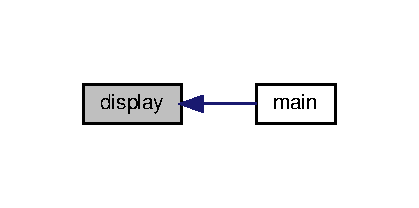
\includegraphics[width=201pt]{user_8c_ac2b3cb6c7ec0748f0c4c1a46e0997d70_icgraph}
\end{center}
\end{figure}
\mbox{\Hypertarget{user_8c_afbdf40ca68538464d0df29d9b2a77366}\label{user_8c_afbdf40ca68538464d0df29d9b2a77366}} 
\index{user.\+c@{user.\+c}!rotate\+\_\+180@{rotate\+\_\+180}}
\index{rotate\+\_\+180@{rotate\+\_\+180}!user.\+c@{user.\+c}}
\subsubsection{\texorpdfstring{rotate\+\_\+180()}{rotate\_180()}}
{\footnotesize\ttfamily void rotate\+\_\+180 (\begin{DoxyParamCaption}\item[{\hyperlink{structcontainer}{container} $\ast$}]{piece }\end{DoxyParamCaption})}



Definition at line 36 of file user.\+c.



References container\+::data, container\+::len, and container\+::size.


\begin{DoxyCode}
37 \{
38     \textcolor{keywordtype}{int} i,j,width,height;
39     width=piece->\hyperlink{structcontainer_a1e938d250074e70b9778df1b59121744}{size}/piece->\hyperlink{structcontainer_a0069496fb95c879cd33fb79ab726e81a}{len};
40     height=piece->\hyperlink{structcontainer_a0069496fb95c879cd33fb79ab726e81a}{len};
41     \textcolor{keywordtype}{char} * tmp=malloc(\textcolor{keyword}{sizeof}(\textcolor{keywordtype}{char})*width*height);
42     \textcolor{keywordflow}{for}(i=0;i<width;i++)
43         \textcolor{keywordflow}{for}(j=0;j<height;j++)
44             tmp[i*width+j]=piece->\hyperlink{structcontainer_aefae69762fe9c24169e2ca5418a711a1}{data}[i+width*j];
45 
46     \textcolor{keywordflow}{for}(i=0;i<width;i++)
47         \textcolor{keywordflow}{for}(j=0;j<height;j++)
48             piece->\hyperlink{structcontainer_aefae69762fe9c24169e2ca5418a711a1}{data}[i*width+j]=tmp[i*width+j];
49     free(tmp);
50 \}
\end{DoxyCode}
\mbox{\Hypertarget{user_8c_a44fa0cbfa7fc79473c8ac9ca3b198f5a}\label{user_8c_a44fa0cbfa7fc79473c8ac9ca3b198f5a}} 
\index{user.\+c@{user.\+c}!rotate\+\_\+90@{rotate\+\_\+90}}
\index{rotate\+\_\+90@{rotate\+\_\+90}!user.\+c@{user.\+c}}
\subsubsection{\texorpdfstring{rotate\+\_\+90()}{rotate\_90()}}
{\footnotesize\ttfamily void rotate\+\_\+90 (\begin{DoxyParamCaption}\item[{\hyperlink{structcontainer}{container} $\ast$}]{piece }\end{DoxyParamCaption})}



Definition at line 52 of file user.\+c.



References container\+::data, container\+::len, and container\+::size.


\begin{DoxyCode}
53 \{
54     \textcolor{keywordtype}{int} i,j,width,height;
55     width=piece->\hyperlink{structcontainer_a1e938d250074e70b9778df1b59121744}{size}/piece->\hyperlink{structcontainer_a0069496fb95c879cd33fb79ab726e81a}{len};
56     height=piece->\hyperlink{structcontainer_a0069496fb95c879cd33fb79ab726e81a}{len};
57     \textcolor{keywordtype}{char} * tmp=malloc(\textcolor{keyword}{sizeof}(\textcolor{keywordtype}{char})*width*height);
58     \textcolor{keywordflow}{for}(i=0;i<width;i++)
59         \textcolor{keywordflow}{for}(j=0;j<height;j++)
60           \textcolor{keywordflow}{if}(j== 0)
61                 tmp[i*width+j]=piece->\hyperlink{structcontainer_aefae69762fe9c24169e2ca5418a711a1}{data}[width*(width-1)+i];
62 
63             \textcolor{keywordflow}{else} \textcolor{keywordflow}{if} (j>0  && j <width)
64                 tmp[i*width+j]=piece->\hyperlink{structcontainer_aefae69762fe9c24169e2ca5418a711a1}{data}[width*j+i];
65             \textcolor{keywordflow}{else} \textcolor{keywordflow}{if}(j == width)
66                      tmp[i*width+j]=piece->\hyperlink{structcontainer_aefae69762fe9c24169e2ca5418a711a1}{data} [width-i];
67 
68     \textcolor{keywordflow}{for}(i=0;i<width;i++)
69         \textcolor{keywordflow}{for}(j=0;j<height;j++)
70             piece->\hyperlink{structcontainer_aefae69762fe9c24169e2ca5418a711a1}{data}[i*width+j]=tmp[i*width+j];
71     free(tmp);
72 \}
\end{DoxyCode}

%--- End generated contents ---

% Index
\backmatter
\newpage
\phantomsection
\clearemptydoublepage
\addcontentsline{toc}{chapter}{Index}
\printindex

\end{document}
